% !TeX spellcheck = <none>
%%%%%%%%%%%%%%%%%%%%%%%%
%Authors: Luis A. Duffaut & Francisco Rosales
%%%%%%%%%%%%%%%%%%%%%%%%

%required packages and operators
% interactcadsample.tex
% v1.03 - January 2017

\documentclass[]{interact}

\usepackage{epstopdf}% To incorporate .eps illustrations using PDFLaTeX, etc.
\usepackage{subfigure}% Support for small, `sub' figures and tables
%\usepackage[nolists,tablesfirst]{endfloat}% To `separate' figures and tables from text if required
\usepackage[numbers]{natbib}% Citation support using natbib.sty
%%% ============================================================================================================= %%%
%%%                                  The lastest updated date: March, 2009                                    %%%
%%% ============================================================================================================= %%%
%%% Update Log: 11/16/2004, add the \RomanNumber and \romannumber for capital and small Roman numbers
%%%                         add \rb for table raising box
%%% Update Log: 05/08/2004, add the matlab and simulink definition in the end for reference
%%% Update Log: 04/26/2004, add the math operator ``dist'', update the definition for theorem-like enviroments
%%% Update Log: 03/04/2004, use package 'upgreek' for constants, e.g., $\uppi$ = 3.1415926.... (ISO standard)
%%% Update Log: 09/12/2004, update for solving the conflicts between amsthm and cssconf
%%% Update Log: 05/03/2009, merging with Luis' abbreviation setting
%%% Update Log: 01/20/2010, adding H option for floating figures
%%% ============================================================================================================= %%%

\usepackage{latexsym, amssymb, amsmath}
%\usepackage[dvips]{graphicx} % added for inserting the pictures

%%%%%%%%%%%%%%%%
\usepackage{float}      %these two packages are for fixing figures in place
\restylefloat{figure}
%%%%%%%%%%%%%%%%

\usepackage{graphicx,dsfont}
\usepackage{mathrsfs}  % package for math fonts: mathscripts \mathscr
\usepackage{color} % standard color package
\usepackage[latin1]{inputenc}
\usepackage{enumerate}
\usepackage{flushend} % align at the last lines of every page
\usepackage{stfloats}
\usepackage{balance}
\usepackage{tabularx}
\usepackage{bm}

%%% Added by LADE

%\usepackage{algorithm}
%\usepackage[noend]{algpseudocode}
\usepackage[linesnumbered,ruled]{algorithm2e}
\usepackage{algcompatible}
%\makeatletter
%\def\BState{\State\hskip-\ALG@thistlm}
%\makeatother


%%%

\bibpunct[, ]{(}{)}{;}{a}{}{,}% Citation support using natbib.sty
\renewcommand\bibfont{\fontsize{10}{12}\selectfont}% Bibliography support using natbib.sty

\theoremstyle{plain}% Theorem-like structures provided by amsthm.sty
\newtheorem{theorem}{Theorem}[section]
\newtheorem{lemma}[theorem]{Lemma}
\newtheorem{corollary}[theorem]{Corollary}
\newtheorem{proposition}[theorem]{Proposition}
\newtheorem{algo}{Algorithm}[section]

\theoremstyle{definition}
\newtheorem{definition}[theorem]{Definition}
\newtheorem{example}[theorem]{Example}

\theoremstyle{remark}
\newtheorem{remark}{Remark}
\newtheorem{notation}{Notation}

\def\begce{\begin{center}}
\def\endce{\end{center}}

\definecolor{colorLADE}{rgb}{1, 0.5, 0}
\def\bluetext#1{\textcolor[rgb]{1.00,0.00,0.00}{#1}}

\begin{document}
\title{Embedding Spatial Variability in Rainfall Field Reconstruction} 

	
\author{
\name{Luis~A.~Duffaut~Espinosa\textsuperscript{a}\thanks{CONTACT Luis~A.~Duffaut~Espinosa. Email:  lduffaut@uvm.edu.}, Francisco Rosales\textsuperscript{b}, and Adolfo Posadas\textsuperscript{c}}
\affil{\textsuperscript{a}Department of 
Electrical and Biomedical Engineering, University of Vermont, 
Burlington, Vermont 05041, USA.; \textsuperscript{b}Academic Department of Finance, Universidad del Pac\'ifico, Av. Salaverry 2020, Lima 11, Per\'u; \textsuperscript{c}Agrosight, Allia Future Business Centre, Kings Hedges Road, Cambridge CB4 9HY, UK.}
}

\maketitle

%abstract%%%%%%%%%%%%%%%%%%%%%%%%%%%%%%%%%%%%%%%%%%%%
\begin{abstract}
	
This manuscript provides a methodology for the reconstruction of a rainfall  field when \bluetext{there are scarce rain-gauge stations available}.  This situation typically arises when measurements are taken from  meteorological stations across time, and the information for the complete field is required as an input for larger scale models. The proposed method is based on a wavelet reconstruction technique that requires no distributional assumptions, but relies on the relation between rainfall and 
NDVI (Normalized Difference Vegetation Index) to account for the unobserved spatial variability of the field. The methodology is applied over a region of the southern Peruvian Andes where data gathered from meteorological stations provide enough  statistical significance. A comparison  with respect to an alternative source of spatial variability and common practices is provided. 
\end{abstract}

\begin{keywords}
Rainfall reconstruction, NDVI, Wavelets. 
\end{keywords}


%section: introduction%%%%%%%%%%%%%%%%%%%%%%%%%%%%%%%%%%%%%%%%%
\section{Introduction}


Rainfall data collected from sparsely distributed meteorological stations is a common scenario faced by climate scientists. Whether it is to be used as an input in climate/weather models or to characterize its behavior in its original scale, a statistical reconstruction method of the signal is of great importance. Hydrological and general circulation models (GCM) are typical examples of this situation, where daily rainfall data is required as input to run simulations under specific scenarios. The results are then used to \bluetext{predict} drought periods or to understand changes in climate systems  \citep{lloyd}.  In fact, there is a pressing need amongst policy makers (e.g. UN, USAID and FAO) for the reconstruction and correction of atmospheric datasets. Currently, these datasets are produced via global and regional models for rainfall outputs as well as  ground/space-based rainfall observations such as those provided by  NASA's earth-observing satellite missions. However, even though these measurements produce information having operational resolutions of $1$ km and finer, their accuracy is at best $10$ km due to the physical limitations such as cloud microphysics and terrain heterogeneity.  \bluetext{These} problems motivate the usage of correction methods \citep{Hwang-Graham_2013}, and alternative reconstruction techniques \citep{Duffaut-et-al_2017,Hartkamp-et-al_99,Heidinger-et-al_2012,Hijmans-et-al_2005,Hutchinson_95,Lovejoy-Schertzer_2013,Price-et-al_2000,Posadas-et-al_2015,Quiroz-et-al_2011}.

The rainfall reconstruction technique proposed in this manuscript can be seen as an statistical method that exploits the well-known \bluetext{linear correlation} between rainfall and the so-called Normalized Difference Vegetation Index (NDVI) in regions where the annual rainfall goes from $200$ to $1200$ mm \bluetext{\cite{Nicholson-et-al_1996,Quiroz-et-al_2011}.  The linearity limit corresponds to regions with low annual precipitations \citep{Martiny-et-al_2006}.} In \citep{Heidinger-et-al_2012,Quiroz-et-al_2011}, a point-wise version of the technique was used on low resolution data obtained from the  Tropical Rainfall Measuring Mission (TRMM) \citep{Simpson-et-al_96}. However, it was found that when the reconstruction was applied on a point (spatial) sufficiently far from a meteorological station,  the reconstruction showed certain bias towards the station and failed to embed the spatial heterogeneity of the surrounding area. The main contribution of the current method is that it  incorporates the spatial heterogeneity of NDVI via: $1)$ a temporal wavelet reconstruction \citep{mallat98},  and $2)$ a spatial prediction \citep{Cressie_91}.


The method is applied to rainfall datasets for the Southern Peruvian Andes with data gathered from meteorological stations sparsely distributed in the region shown in Figure \ref{fig:study_area}, and it is tested with relevant competing methods such as ANUSPLIN interpolation and wavelet-based closest station correction \citep{Quiroz-et-al_2011}. The results show that the proposed method provides an improvement over common practices in that it gives better statistical metrics  and goodness of fit of exceedance curves. It also remove fictitious boundaries introduced by Thiessen polygons when the rainfall influence at a spatial point is assumed to correspond to the closest meteorological station. 

The structure of the manuscript is as follows. Section $2$ describes the region of study and the datasets. Section $3$ presents some mathematical tools, and the reconstruction method  is discussed in terms of two algorithms. In Section $4$ the method is applied to rainfall data collected from the southern Peruvian Andes, its performance is compared to other   methods available in the literature, and the results are discussed.  Section $5$ provides conclusions and points of interest for future research.  

%section: empirical%%%%%%%%%%%%%%%%%%%%%%%%%%%%%%%%%%%%%%%%%
\section{Region of Study and Data}

\subsection{Study area} \label{subsubsec:2_1}
The studied region is defined by a grid with $225\times225$ cells of approximately 
$1$km$^2$ each from  the Southern Peruvian Andes (Figure \ref{fig:study_area}). The 
majority of these cells are placed in the Peruvian Andean High-plateau or 
Altiplano, and a few cells, over the East side of the Andes. Geographical 
coordinates of the study area are between latitudes $14^\circ$ to $16^\circ$ 
South and longitudes $69^\circ$ to $71^\circ$ West {constituting an area of 
approximately $225\times 225$ {km}$^2$}. The altitudes range between $800$ 
to $6500$ {m.a.s.l}, approximately. The annual rainfall varies, on 
average, from $\sim 250$ {mm} in the arid southwest to $\sim 5000$ {mm} in the 
Amazon basin at the northeast corner of the study site 
\citep{Garreaud-et-al_2003}. {In this area of study, there are $19$ 
meteorological stations from which observed rainfall measurements are obtained 
during a period of $8$ years (from $1999$ to $2006$). \bluetext{ 
The meteorological station data was obtained from the official Peruvian meteorological agency \citep{Senamhi}, which reports daily aggregations from tipping bucket rain gauges at $0.1$ mm resolution. The measurements provided by SENAMHI amount to time series having $1$ day temporal resolution.} 

\subsection{Data}\label{subsubsec:2_2}

The main source of information for the methodology developed in section \ref{sec:3} is NDVI data. The NDVI dataset consists of $288$ (dekad) composite images 
{($225\times 225$ pixels) with an approximate resolution of $1$ km 
corresponding to the area} shown in Figure~\ref{fig:study_area}. \bluetext{NDVI data here correspond to the product VGT-S10 NDVI, which} is derived from the vegetation instruments SPOT-$4$ and SPOT-$5$ over the time period starting in January $1999$ and ending in December $2006$. The period from January $2007$ to December $2007$ is also considered in this work for 
correction purposes \citep{Quiroz-et-al_2011}.  The spectral and spatial 
resolution of the vegetation instruments is the same. The spectral band 
$0.61$-$0.68$ mm corresponding to red (${R}_{\mbox{\tiny Red}}$), and the band $0.78$-$0.89$ mm corresponding 
to near-infrared (${R}_{\mbox{\tiny Infrared}}$) were used to compute the NDVI index by employing the 
standard formula  
\begin{align} \label{eq:NDVI_definition}
\mbox{NDVI}= \frac{{R}_{\mbox{\tiny Infrared}} - {R}_{\mbox{\tiny Red}}}{{R}_{\mbox{\tiny Infrared}} + {R}_{\mbox{\tiny Red}}}.
\end{align}
The final product has a spatial resolution of $\sim1$ km. The above 
formula for the NDVI index restricts the values to be in the interval 
$[-1,1]$. In addition, the NDVI index is geometrically and radiometrically 
corrected producing the $S10$ NDVI product \citep{Immerzeel-et-al_2005}. \bluetext{The 
dates assigned to the $288$ dekadal samples were defined according to the civil 
calendar. In particular,} every month was divided into $3$ pieces: from the $1$st day to the $10$th; from the $11$th to the $20$th; and from the $21$st to the end of each month. Each month therefore produces $3$ NDVI data points per month \bluetext{for which the maximum value of NDVI in each piece of the month is assigned to the $10$th, $20$th and last day of the month.} \bluetext{Since  the NDVI product used in this paper is not evenly sampled, NDVI data has been re-sampled to an uniformly sampled $8$ day resolution prior to its lag correction as described in \citep{Duffaut-et-al_2017} given the inherent smoothness of the data. The $8$ day resolution was chosen since it is convenient for the wavelet technique used in Section~\ref{sec:3}.} In addition, NDVI contains a temporal lag with respect to the precipitation at a particular instant of time. \bluetext{The lag in the NDVI signal is the latency time that takes between rainfall reaching the ground and the time changes in the biomass index are registered in the red and infrared frequencies \citep{Tucker_79}.} The developments in \bluetext{\citep{Immerzeel-et-al_2005,Yarleque-et-al_2016} and \citep[Section $4$]{Duffaut-et-al_2017} were} followed in order to correct for this NDVI lag response, and therefore the NDVI dataset used in this paper accounts already for lag correction \bluetext{and re-sampling to a uniform $8$ day resolution.}  \bluetext{To synchronize the time resolutions of the NDVI data and the ground measurements, the daily ground measurements were added every $8$ days and the accumulated value is assigned at the end of each $8$ day period.}



A second source of information is obtained from the interpolation of the $19$ meteorological stations data using the thin-plate smoothing spline algorithm implemented in the ANUSPLIN $4.36$ package  \citep{Hutchinson_2006,ANUSP_07}. This interpolation considers the latitude, longitude, and elevation of the area in addition to measured rainfall at each station \citep{Hutchinson_95}. The method was chosen due to its higher accuracy compared to other methods in areas similar to the Andes high plateau, see 
\citet{Hijmans-et-al_2005,Hartkamp-et-al_99,Jarvis-Stuart_2001, 
Price-et-al_2000}. We also justify this selection since  several climate products such as WorldClim (\citep{Hijmans-et-al_2005},\citep{worldclim}) and IWMI Climate 
Atlas/CRU gridded data (\citep{New-et-al_2002}, \citep{IWMI}, 
\citep{UEACRU}) have successfully applied the ANUSPLIN methodology. 

%section: methods%%%%%%%%%%%%%%%%%%%%%%%%%%%%%%%%%%%%%%%%%
\section{Methods}\label{sec:3}

Let $Y(s,t)$ denote a  rainfall field, where  $s\in\mbox{S}$ with $\mbox{S}$ denoting the set of all spatial coordinates of $Y$, $t\in\mbox{T}$ with $\mbox{T}$ denoting the set of all times related to $Y$ at which the measurements are taken. Consider that $Y$ is only known for $s\in\{s_1,s_2,\dots\}\subset\mbox{S}$ and $t\in\{t_1,t_2,\dots\}\subset\mbox{T}$, and that one is interested in  estimating $Y$ for all other $s\in\mbox{S}$ and  $t\in\mbox{T}$. This situation typically arises in climate science when data is measured only at certain locations where there are meteorological stations and during certain period of time. However, climate modelers require information for the complete sets $\mbox{S}$ and $\mbox{T}$, for instance, as input for models such as general circulation models (GCM) or hydrology \bluetext{transport} models that require either better spatial and/or time resolutions.  This is achieved by introducing auxiliary information in order to complete the unknown values of $Y$. 

In what follows the field $Y(s,t)$ is handled fixing one of its two components. When this is the case, a bar will be placed above the component that is meant to be fixed. For example, $\text{\boldmath$Y$}(\bar{s},t)$ denotes a time series vector, while $\mbox{\textbf{Y}}(s,\bar{t})$  denotes a day sample matrix of the field at time $\bar{t}$ (spatial point process). 

\subsection{Temporal wavelet reconstruction} \label{subsubsec:3_1}

\subsubsection{Wavelet transforms}
The wavelet transform of a function $f(t)$ with finite energy is defined as the integral transform with a family of functions	
$\psi_{\lambda,t}(u):=\frac{1}{\sqrt{\lambda}}\psi\left(\frac{u-t}{\lambda}\right)$, and it is given by
\begin{eqnarray}
\langle f,\psi_{\lambda,t}\rangle&=&\int_{-\infty}^\infty f(u)\psi_{\lambda,t}(u){\rm{d}}u,\quad\lambda>0\\ 
			&=&\int_{-\infty}^\infty f(u)\frac{1}{\sqrt{\lambda}}\psi\left(\frac{u-t}{\lambda}\right){\rm{d}}u,
\end{eqnarray}
where   $\lambda$ is a scale parameter, $t$ a location parameter and the functions $\psi_{\lambda,\tau}$ are called wavelets. The inverse wavelet transform is given by
\begin{eqnarray}
f(t)&=&\frac{1}{{\cal C}_\psi}\int_{-\infty}^\infty\int_{0}^\infty\lambda^{-2}Wf(\lambda,u)\psi_{\lambda,u}(t){\rm{d}}\lambda {\rm{d}}u,\\
{\cal C}_\psi&=&2\pi\int_{0}^\infty\frac{|\hat\psi(\omega)|^2}{\omega}{\rm{d}}\omega<\infty,
\end{eqnarray}
where $Wf(\lambda,u):=\langle f,\psi_{\lambda,u}\rangle$, $\hat{\psi}$ is the Fourier transform of $\psi$ and $\omega$ is the frequency variable in the Fourier domain.\\

%discrete wavelet transform
When the parameters $\lambda$  and $t$ in the wavelet transform $\langle f,\psi_{\lambda,t}\rangle$ lie in a continuum, the transform it is called continuous wavelet transform. To obtain a discrete wavelet transform one can choose  choose   $\lambda=\lambda_0^m$, where $m$ is an integer and $\lambda_0>1$ is a fixed dilation step. In particular, the following discretization is considered:  $t=nt_0\lambda_0^m$, where $t_0>0$, and $n$ is an integer. We can then
re-parametrize the wavelet in terms of $m$ and $n$ as
\begin{eqnarray}
\psi_{m,n}(t)&=&\frac{1}{\sqrt{\lambda_0^m}}\psi\left(\frac{t-nt_0\lambda_0^m}{\lambda_0^m}\right)\\
		&=&\lambda_0^{-m/2}\psi\left(\lambda_0^{-m}t-nt_0\right),
\end{eqnarray}
and the discrete wavelet transform reads:
\begin{equation}
\langle f,\psi_{m,n}\rangle=\lambda_0^{-m/2}\int f(t)\psi\left(\lambda_0^{-m}t-nt_0\right){\rm{d}}t.
\end{equation}

\subsubsection{Wavelet approximation}
Using wavelets that form a complete orthonormal basis (for instance, Haar wavelets), any finite energy function can be approximated up to arbitrary precision by a linear combination of basis functions $\psi_{m,n}(t)$. That is,
\begin{equation}
f(t)  = \sum_{m=-\infty}^\infty\sum_{n=-\infty}^\infty D_{m,n}\psi_{m,n}(t),
\end{equation}
where $D_{m,n}:=\langle f,\psi_{m,n}\rangle =\int_{-\infty}^\infty f(t)\psi_{m,n}(t)dt$. 
Moreover, by using an intermediate scale $m_0$, the last equation can be broken up into two sums
\begin{equation}\label{deco0}
f(t)=\sum_{m=-\infty}^{m_0}\sum_{n=-\infty}^\infty\langle f,\psi_{m,n}\rangle\psi_{m,n}(t)+
\sum_{m=m_0+1}^\infty\sum_{n=-\infty}^\infty\langle f,\psi_{m,n}\rangle\psi_{m,n}(t). 
\end{equation}
If in addition one considers the scaling functions $\phi_{m,n}(t)$ satisfying $\phi_{m,n}(t)=2^{-m/2}\phi(2^{-m}t-n)$ and following the arguments in \citep{fofu}, then it can be shown that 
\begin{equation}
\sum_{m=m_0+1}^\infty\sum_{n=-\infty}^\infty\langle f,\psi_{m,n}\rangle\psi_{m,n}(t)=
\sum_{m=-\infty}^\infty\langle f,\phi_{m_0,n}\rangle\phi_{m_0,n}(t),
\end{equation}
which, in fact, portrays the  low frequency information \bluetext{(LFI)} carried by the signal, \bluetext{whereas the first summation in the right hand side of \eqref{deco0} contains the high frequency information (HFI) of the signal}. To make this separation clear, hereafter the following notation is used for the mentioned decomposition:
\begin{eqnarray}
f(t)&=&L_f(t)+H_f(t) \label{eq:Wav_decomp}\\
H_f(t)&=&\sum_{m=-\infty}^{m_0}\sum_{n=-\infty}^\infty\langle f,\psi_{m,n}\rangle\psi_{m,n}(t)\\
L_f(t)&=&\sum_{m=-\infty}^\infty\langle f,\phi_{m_0,n}\rangle\phi_{m_0,n}(t).
\end{eqnarray}
An iterative decomposition can now be performed. Let $f^0:= f (= L_f+H_f)$ and make $f^1:= L_f$. Perform decomposition \eqref{eq:Wav_decomp} on $f^1$ and make $f^2:= L_{f^1}$. The procedure can be continued an arbitrary number of times as long as the scale parameter allows it. The reverse process is known as \emph{reconstruction} of the signal. That is, at decomposition level $\ell $, the signal $\hat{f}^{\ell -1} := L_{f^{\ell }}+H_{f^{\ell }}$. The procedure is continued at level $\ell -2$ by making $\hat{f}^{\ell -2} := \hat{f}^{\ell -1}+H_{f^{\ell -1}}$, and then repeated until reaching level $0$. Note that signals $f$ and $\hat{f} := \hat{f}^0$ are not necessarily the same, which makes decomposition and reconstruction noncomutative operations.  


Recall that for a rainfall field $X(s,t)$ the variable $s$ denotes the spatial coordinates of the field and $t$ denotes the temporal variable of the field. Suppose there are two fields $X$ and $Z$ related to some climate variable (e.g., rainfall). The field $X$  provides reliable information of the \bluetext{LFI} of such climate variable whereas the field $Z$ carries only information of the \bluetext{HFI} of the same climate variable (e.g., $X$ and $Z$ are datasets obtained  from two different satellite sensors). Therefore, decomposing $\text{\boldmath$X$}(\bar{s},t) = \text{\boldmath$L_X$}(\bar{s},t)+\text{\boldmath$H_X$}(\bar{s},t)$ and $\text{\boldmath$Z$}(\bar{s},t) = \text{\boldmath$L_Z$}(\bar{s},t)+\text{\boldmath$H_Z$}(\bar{s},t)$ at a fixed $\bar{s} \in \mbox{S}$ allows one to reconstruct a signal \text{\boldmath$Y$} at the same location by only using the good information of both sources. That is,   
\begin{equation}
\text{\boldmath$Y$}(\bar{s},t) = \text{\boldmath$L_X$}(\bar{s},t) +\text{\boldmath$H_Z$}(\bar{s},t).	
\end{equation}
The reconstruction procedure can be performed after several levels of decomposition as described in the previous paragraph, which provides a proper embedding of the scaling properties of signals \text{\boldmath$X$} (\bluetext{LFI}) and \text{\boldmath$Z$} (\bluetext{HFI}). The level of decomposition is given by a number $\underline{\ell} \in \mbox{N}$ indicating the level at which the \bluetext{LFI} of \text{\boldmath$X$} and \text{\boldmath$Z$} are closest to each other with respect to some statistical metric.  Algorithm $1$ summarizes the reconstruction procedure using two sources of information, and it is referred here simply as \emph{temporal reconstruction} since it only conveys the time variable of the signals.  

\vspace*{0.1in}
\begin{algorithm}[t]
\SetKwInOut{Procedure}{Proc}
\SetKwInOut{Input}{input}
\SetKwInOut{Output}{output}	
\SetKwInOut{Define}{define}
\Input{$\bar{s}\in \mbox{S}$, $\text{\boldmath$X$}(\bar{s},t)$ and $\text{\boldmath$Z$}(\bar{s},t)$}
\Output{$\text{\boldmath$Y$}(\bar{s},t)$}
\Define{$\textit{$\ell $} \gets \text{current  decomposition level}$, $\bar{\ell} \gets \text{maximum allowed } \ell $,  $\text{\boldmath$X$}^{\ell } \gets \text{\boldmath$X$}(\bar{s},t) \text{ signal at level } \ell $, ${\text{\boldmath$Z$}}^{\ell } \gets \text{\boldmath$Z$}(\bar{s},t)  \text{ signal at level } \ell $, $\rm{dist}  \gets \text{statistical metric between signals}$.}
\begin{algorithmic}[1]
    \STATE $\underline{\ell}\gets 0$
	\FOR{$\ell \leftarrow 0$ \KwTo $\bar{\ell}$}
	\STATE  Decompose $\text{\boldmath$X$}^{\ell } \rightarrow  \text{\boldmath$L_X$}^{\ell } + \text{\boldmath$H_X$}^{\ell }$.
	\STATEx $\;\,\,$ Decompose ${\text{\boldmath$Z$}}^{\ell } \rightarrow \text{\boldmath$L_Z$}^{\ell } + \text{\boldmath$H_Z$}^{\ell }$.
	\STATEx $\;\,\,$ Assign ${\text{\boldmath$X$}}^{\ell +1} \gets \text{\boldmath$L_X$}^{\ell } $
	\STATEx $\;\,\,$ Assign ${\text{\boldmath$Z$}}^{\ell +1} \gets \text{\boldmath$L_Z$}^{\ell } $.
	\IF{$\rm{dist}(\text{\boldmath$X$}^{\ell +1},\text{\boldmath$Z$}^{\ell +1}) < \rm{dist}(\text{\boldmath$X$}^{\ell },\text{\boldmath$Z$}^{\ell })$}
	\STATE $\underline{\ell}=\ell +1$ 
	\ELSE
	\STATE { continue}
	\ENDIF
\ENDFOR
%\algstore{myalg}
%\end{algorithmic}
%\end{algorithm}
%
%\begin{algorithm}                     
%\begin{algorithmic} [1]                   % enter the algorithmic environment
%\algrestore{myalg}
	\FOR{$i\leftarrow 0$ \KwTo $\underline{\ell}$}
	\STATE Reconstruct $\text{\boldmath$Y$}^{i} \gets \text{\boldmath$L_X$}^{i} + \text{\boldmath$H_Z$}^{i}$.
\ENDFOR
 \STATE Return $\text{\boldmath$Y$} \gets \text{\boldmath$Y$}^0$ 
\end{algorithmic}
		\caption{Temporal Reconstruction}
\end{algorithm}
\vspace*{0.1in}


In \citep{Heidinger-et-al_2012}, $\text{\boldmath$X$}(\bar{s},t)$   $\bar{s}\in \mbox{S}$ was taken as the time series obtained from satellite information of The Tropical Rainfall Measuring Mission (TRMM), and $\text{\boldmath$Z$}(\bar{s},t)$  was provided from the closest meteorological station rainfall time series to the location $\bar{s}$. However, the spatial resolution of TRMM data is approximately $28$ km, which, as reported in \citep{Heidinger-et-al_2012} introduces high spatial biases and does not take into account the spatial heterogeneity of the area.  

In this manuscript, a natural candidate for  the field  $X$ that provides a $1$ km resolution is NDVI; while $Z$ is obtained from two sources. The first is based on spline approximations of a finite number of local meteorological stations constructed using the topography map, longitude and latitude  of the area. The main issue of using splines in this context is that splines are inherently smooth whereas rainfall fields exhibit \bluetext{spatial} roughness \citep{Kedem-Long_87,Lin_78}. In the next section, it is argued that a linear predictor of the rainfall \bluetext{HFI} based on a weighted sum of the surrounding meteorological stations  provides a practical improvement over using splines or the closest meteorological station as the $Z$ rainfall field. \bluetext{This amounts to a deterministic reconstruction model that preserve the temporal ($8$ days) and spatial ($1$ km) resolutions of the data.}


\subsection{Spatial reconstruction}

{Two methodologies introducing spatial variability to the methodology in  
\citep{Heidinger-et-al_2012,Quiroz-et-al_2011} are proposed. The first 
one (SR1) involves applying algorithm $1$ to $X=\mbox{NDVI}$ and $Z$ the rainfall field of spatially interpolated meteorological stations via splines  \citep{ANUSP_07,Hutchinson_95,Hutchinson_2006}. Although the rainfall fields obtained from the spline procedure are inherently \emph{smooth} (spatially),  \bluetext{these can still be used to extract the HFI component of the time series  at each point in the area of study  while NDVI, which is inherently smooth (temporally), provides the LFI part}. A comparison of the spatial distribution  between NDVI and ANUSPLIN fields is shown in Figure \ref{fig:NDVI_ANUSLINE} for \bluetext{28 January 2000} at the Andean region. The second methodology (SR2) considers HFI in time at every spatial point in the area of study as a weighted linear combination of all point-wise meteorological stations and the \bluetext{LFI} is provided by $X=\mbox{NDVI}$ information. Specifically, at a location $\bar{s}\in \mbox{S}$ and given that there is only knowledge of information at a finite number of places surrounding $\bar{s}$ (corresponding to meteorological stations locations), an estimation of rainfall is given by the linear predictor
\begin{equation} \label{eq:XhatLambda}
\hat{\text{\boldmath $X$}}(\bar{s},t)= \sum_{i=1}^K \lambda_i \text{\boldmath$X$}_{i}(t),
\end{equation}
where $\lambda_i $ is a weight corresponding to the influence of the $i$th station around $\bar{s}$ and $\text{\boldmath $X$}_i(t)$ represents rainfall measured in time at the $i$th meteorological station. Naturally, these weights must add to $1$, and they depend on their relative \emph{distance} (Euclidean) of $\bar{s}$ to the meteorological stations. Thus, the weights $\{\lambda_i\}_{i=1}^{n}$ are calculated using a procedure borrowed from the \emph{Kriging} interpolation procedure \citep{Cressie_91,Goovaerts_97,Matheron_65}. In this manner,  one can calculate $\hat{\text{\boldmath$X$}}(\bar{s},t)$ for every $\bar{s}\in \mbox{S}$, and  the rainfall field containing the high frequency in algorithm $1$ is $Z = \hat{X}$. 
}

\subsubsection{Weight calculation}

Calculating the weights in \eqref{eq:XhatLambda} requires spatial information of the area under study. A good source of spatial information is $X=\mbox{NDVI}$ due to its $1$ km spatial resolution. The first step is then to compute the 
semivariogram of $\mbox{\textbf{X}}(s,\bar{t})$ for a fixed time $\bar{t}\in \mbox{T}$. This provides a notion of a zone of influence for the meteorological stations at  each location in the area. Omitting time dependence,  the experimental semivariogram is computed as
\begin{equation}
 \gamma(h) = \frac{1}{2 {\cal K}(h)}\left(\sum_{\|s_j-s_i\|_2=h}({{X}}(s_j,\bar{t}) - {{X}}(s_i,\bar{t}))^2\right), 
\end{equation}
where $\|\cdot\|_2$ denotes the Euclidean norm, $h$ is the separation distance between locations $s_i$ and $s_j$,  ${\cal K}(h)$ is the number of location pairs separated by $h$, and $\mbox{\textbf{X}}(s_i,\bar{t})$ is the value of the information (NDVI) at location $s_i\in \mbox{S}$ \citep{Cressie_91}. For simplicity, only isotropic semivariograms are considered, however the information in heterogeneous terrain is very likely to be anisotropic. \bluetext{For illustration purposes,} Figure \ref{fig:semivariance} shows the averaged (in time) experimental semivariogram, \bluetext{which gives an idea of the average shape of a semivariogram obtained from an arbitrary NDVI day sample.} 
The experimental semivariogram is then fitted to the function
\begin{equation}
\gamma(h) = \left\{\begin{array}{rl} 
 r+ (c-r)\left\{ \frac{3}{2}\left(\frac{ h}{a}\right)- 
\frac{1}{2}\left(\frac{h}{a}\right)^3\right\} , & h\ge a   \\ c, & 
\mbox{otherwise} \end{array}\right.
\end{equation}
where $c$ is the \emph{sill}, $a$ is the range, and $r$ is the nugget effect 
parameter \citep{Cressie_91}. 
\bluetext{The results in Section~\ref{sec:4}  utilize only the semivariogram corresponding to the same NDVI day sample.}

The task now is to find the explicit relationship between an arbitrary location $\bar{s}\in \mbox{S}$ and $K$ fixed locations $\{\bar{s}_1,\ldots,\bar{s}_K\}\in\mbox{S}$.  Assuming that NDVI  is constituted as a random field that is weakly stationary whose mean $\mu$ and covariance function $C(i,j)$ with respect to the $K$ fixed locations can be estimated from the data, then one can find the best linear relationship between NDVI at $\bar{s}$ and NDVI at the $K$ fixed locations. That is,  the linear predictor   
\begin{equation}
X(\bar{s},\bar{t}) = \sum_{i=1}^K \lambda_i X(\bar{s}_i,\bar{t}),
\end{equation}
where $X(\bar{s}_i,\bar{t})$ is the value of the  field at location $\bar{s}_i$ and time $\bar{t}$. The weights $\lambda_i$ are thus computed so that they minimize the mean squared 
error 
\begin{eqnarray} 
e & =& \mathbb{E}\left[\left(X(\bar{s},\bar{t}) - \sum_{i=1}^K \lambda_i  X(\bar{s}_i,\bar{t})\right)^2\right] \\
& =& {\rm{Var}}\left(X(\bar{s},\bar{t}) - \sum_{i=1}^K \lambda_i X(\bar{s}_i,\bar{t}) \right) \\
& =& C(0,0)-2 \sum_{i=1}^K \lambda_i C(0,j) + \sum_{i=1}^K\sum_{j=1}^K \label{eq:min_MSE_kriging}
\lambda_i \lambda_j C(i,j).
\end{eqnarray}
Note that $C(i,j)$ is just the $(i,j)$ element of the covariance matrix with respect to locations $\{\bar{s}_1,\ldots,\bar{s}_K\}$, and 
that the value $C(0,i)$ is the correlation of the location $\bar{s}$ with respect to location $\bar{s}_i$. It is now only a matter of taking the derivative of $e$ with respect to each $\lambda_k$. That is,
\begin{equation}
 \frac{{\rm{d}} \,e}{{\rm{d}} \lambda_k} = -2 C(0,k) +2\lambda_k C(k,k) + 2 \sum_{i\neq k}^K
\lambda_i C(i,k) = 0,\quad   k=1,2, \ldots,K,
\end{equation}
and since $C(i,j)=C(j,i)$ it follows that
\begin{equation} \label{eq:covariance_equation}
\left(\begin{array}{c} C(0,1)\\ \vdots \\ C(0,K) 
\end{array}\right) = \left(\begin{array}{ccc} 
C(1,1) & \cdots & C(1,K) \\ \vdots & \ddots & \vdots \\ C(N,1) & \cdots & C(N,K) 
\\ \end{array}\right) \left(\begin{array}{c} 
\lambda_1\\ \vdots \\ \lambda_K \end{array}\right).
\end{equation}
Define $\bm{b} = ( C(0,1) \cdots C(0,K) )^\top$, ${\bf C} = \{C(i,j)\}_{1 \le i,j \le K}$ and $\bm{\lambda} = ( \lambda_1 \cdots \lambda_K )^\top$. Solving for $\bm{\lambda}$ in \eqref{eq:covariance_equation} yields
\begin{equation} \label{eq:lambdaKRIG}
{\bm{\lambda}}= {\bf C}^{-1}{\bm{b}},  
\end{equation}
which only depend on the covariance matrix values. The values of $\bm{b}$ and ${\bf C}$ 
can be directly obtained from the semivariogram computed out of the time 
averaged NDVI information since 
$
C(h) = C(0) - \gamma(h), 
$
where $C(h) := C(i,j)$ such that $||s_i-s_j||=h$ and $C(0)$ is the variance at the point of interest $\bar{s}$ \citep{Cressie_91}. Furthermore, one also require that  $\sum_{i=1}^n \lambda_i=1$ so that the system becomes 
\begin{equation}
\left(\begin{array}{c} C(0,1)\\ \vdots \\ C(0,K) \\1
\end{array}\right) = \left(\begin{array}{cccc} 
C(1,1) & \cdots & C(1,K) & 1 \\ \vdots & \ddots & \vdots & \vdots \\ C(N,1) & 
\cdots & C(N,K) & 1 \\ 1 & \cdots & 1 & 0  \end{array}\right) 
\left(\begin{array}{c} 
\lambda_1\\ \vdots \\ \lambda_K \\ \eta \end{array}\right),
\end{equation}
where $\eta$ is a \emph{Lagrange Multiplier}. 
% From the procedure described above, one can easily find that the optimal Kriging variance is then 
% \begin{equation} \label{eq:krigingvarianceequation}
%  \sigma^2 = C(0,0) -\sum_{i=1}^K C(0,i).
% \end{equation}
Since matrix {{$\bf{C}$}} can be singular, the pseudo inverse of ${\bf C}$ is used instead of the inverse. This fact, and numerical errors amounts for the possibility of having values of lambda slightly over $1$, which at the same time causes other lambda values (corresponding to the same location) to be negligibly negative. Clearly, this is a consequence of the condition that forces  the sum of weights to be equal to $1$. 

\subsubsection{Reconstruction algorithm}

{The computation of weights presented in the previous section have to be performed for all times $t\in\mbox{T}$. This provides a complete set of day samples containing the region of influence of each of the $K$ locations where there is full rainfall information taken at meteorological stations. It is thus that one can compute the field $\hat{X}$ as a function of time and space via \eqref{eq:XhatLambda}. Finally, Algorithm $1$ is applied  $X = \mbox{NDVI}$ and $Z=\hat{X}$. The overall process is described in Algorithm $2$.  \\

\begin{algorithm}[t]
	\SetKwInOut{Procedure}{Proc}
	\SetKwInOut{Input}{input}
	\SetKwInOut{Output}{output}	
	\SetKwInOut{Define}{define}
	
	\Input{$X$ and $Z$}
	\Output{$Y$}
	
	
	\begin{algorithmic}[1]
		\FOR{$\bar{s} \in \mbox{S}$}
		\STATE  compute $\{\lambda_1(\bar{s}),\ldots,\lambda_K(\bar{s}) \}$ using \eqref{eq:lambdaKRIG} for all $ t\in\mbox{T}$,
		\STATE  compute $\hat{\text{\boldmath$X$}}(\bar{s},t)$ using  \eqref{eq:XhatLambda},
		\STATE apply  Algorithm $1$ to find $\text{\boldmath$Y$}(\bar{s},t)$ with $\text{\boldmath$X$}(\bar{s},t) =  \mbox{NDVI}(\bar{s},t)$ and 
		\STATE $ \text{\boldmath$Z$}(\bar{s},t) = \hat{\text{\boldmath$X$}}(\bar{s},t)$		
		\ENDFOR
		\STATE Return $Y(s,t)$ for all $s\in \mbox{S}$ and $t\in\mbox{T}$ 
	\end{algorithmic}
	\caption{Spatial Reconstruction}
\end{algorithm}
}


%section: Results%%%%%%%%%%%%%%%%%%%%%%%%%%%%%%%%%%%%%%%%%
\section{Results and Validation}  \label{sec:4}

Methodologies SR1 and SR2 based on algorithms $1$ and $2$ and described in section \ref{sec:3} are now applied to the region of the Andes high plateau shown in Figure \ref{fig:study_area}. 


\subsection{Results}

A key calculation for algorithms $1$ and $2$ is computing the decomposition level $\underline{\ell}$. As described in Algorithm $1$, $\underline{\ell}$ is computed by comparing the low frequency components of NDVI and either spline interpolation using the ANUSPLIN software (SR1) or $\hat{X}$ obtained using \eqref{eq:XhatLambda} (SR2). Then $\underline{\ell}$ is the level that provides a better goodness of fit statistic. That is, the statistical metric $\rm{dist}$ is chosen to be either the Nash-Sutcliffe Efficiency or the correlation coefficient.  For the SR1 methodology, Figure \ref{fig:level_decomposition1} shows $6$ levels of decomposed NDVI and ANUSPLIN time series for location ($50$,$160$) in the grid of $225\times 225$ cells covering Figure \ref{fig:study_area} with location ($0$,$0$) being the upper left corner of the figure. Figure \ref{fig:level_decomposition5} shows $6$ levels of decomposition for the SR2 methodology where NDVI and $\hat{X}$ obtained using the weighted linear predictor are compared. Tables \ref{table:ANUSP_goddness_50_160} and \ref{table:Krig_goddness_50_160} show the goodness of fit statistics for the time series at this point used in selecting $\underline{\ell}$ for SR1 and SR2, respectively. At location ($200$,$20$) in the grid, the decomposition levels are shown in Figures \ref{fig:level_decomposition2} and \ref{fig:level_decomposition5} as well as the corresponding goodness of fit statistics in Tables \ref{table:ANUSP_goddness_200_20} and \ref{table:Krig_goddness_200_20}  for the  SR1 and SR2 methodologies, respectively. From these tables, it is clear that $\underline{\ell}$ is either $3$ or $4$. In general, it was observe that the level of decomposition for all grid points falls between levels $3$ and $4$, \bluetext{corresponding to a time dilation of $64$ and $128$ days, respectively. These time resolutions are within the range of NDVI lags reported for the studied region in \citep{Duffaut-et-al_2017,Yarleque-et-al_2016}. \bluetext{Levels $3$ and $4$ are highlighted in Tables  \ref{table:ANUSP_goddness_50_160} to \ref{table:Krig_goddness_200_20} to show that these are always the ones providing the optimal level of decomposition needed for applying the temporal reconstruction described in algorithm $1$.} That is, the maximum value of the goodness of fit descriptors (Nash-Sutcliffe and correlation coefficient) correspond to level $3$ or $4$.} Therefore, a  reasonable choice for $\underline{\ell}$ for all locations in the grid is assumed to be $3$. 



The SR1 methodology employs the $19$ meteorological stations in the area of study as reference points to compute a $225\times 225 \times 288$ dataset of rainfall values using the ANUSPLIN software. Then algorithm $2$ is applied directly. For the SR2 methodology, the same $19$ meteorological stations are used for the calculation of the field $\hat{X}$ with  weights computed using the spatial information provided by the NDVI dataset. Figure \ref{fig:LambdaImages} shows the weights of $4$ particular stations. Note that the spatial distribution of the weights provides a notion of the range of influence of meteorological stations.  The results of the reconstructed rainfall are showed in Figure \ref{fig:3methodsComparison} for $4$ randomly chosen days during the $8$ year period of available NDVI information. The left column gives  the results of using the SR1. The right column shows the result of the SR2 methodology. For 
comparison purposes, the middle column shows the case in which $\hat{X}$ at a specific location is given by the single closest meteorological station to the location of interest. Note that the area of influence in this case becomes the well-known Thiessen polygons \citep{Voronoi_1908}. It is observed in this case that there is a  clear bias with respect to the station at the centre of each 
polygon, which produces an obvious fictitious rainfall boundary with the same shape of the Thiessen polygons.  

\subsection{Validation}

Given that the reconstruction algorithms employs MRA on time series, a temporal 
validation on two grid points in the region is performed. For this 
purpose, two meteorological stations in the region of study were kept out of 
the process for generating ANUSPLIN and $\hat{X}$ fields. From this perspective, the validation is unbiased towards the algorithms $1$ and $2$. These stations are 
Pucara and Santa Rosa. Pucara is geographically located at longitude 
\bluetext{$70.37^\circ$ W, $15.03^\circ$ S} and Santa Rosa is at \bluetext{$70.79^\circ$ W, $14.62^\circ$ S} both have an altitude above $3900$~{m.a.s.l}. Pucara and Santa Rosa stations were picked due to the fact that they are located on heterogeneous terrain and therefore they are representative of the spatial variability of the area. 

Figure \ref{fig:PucStaRosTimeSeries} shows the comparison of the data measured 
and data reconstructed at Pucara and Santa Rosa stations, and the corresponding statistics are shown in Table 
\ref{table:PucStaRosaTimeseriestable}, where one notices the good agreement of 
the Hurst index, mean, maximum value, quantiles and variance. The 
discrepancies can be attributed to the stochastic nature of the 
time series as well as the difference in spatial scales. \bluetext{For example, the Hurst index being close to $0.5$ indicates that there is not much correlation between the current and future observations, which is also indicated by the reconstructed time series.} The exceedance probability curves were also computed and shown in Figure  
\ref{fig:3methodsComparison3}. This is validated by the goodness of fit statistics provided in Table \ref{table:PucStaRosaTimeseriesGoF} only for the weighted reconstruction procedure. The table shows the following indicators of the goodness of 
fit: MAE (mean average error) , RMSE (root mean squared error), CORR (correlation coefficient), PBIAS (Percent Bias), NSE (Nash-Sutcliffe Efficiency) and RSR (ratio of RMSE to the standard deviation of the observations). As a rule of thumb, the fitting or reconstruction can be considered satisfactory if the indicator NSE is greater than $0.50$ and the indicator RSR is around $0.80$ or below. This is indeed the case for both 
stations; see Table \ref{table:PucStaRosaTimeseriestable}. In addition, one 
can clearly see that the exceedance curves for the reconstructed NDVI data 
overlap better with the observed exceedance curves in comparison with the 
reconstructed curves obtained using spline interpolations. \bluetext{Discrepancies and errors are expected in this application. Some reasons for that can be attributed to the nature of NDVI in that it is a ratio of spectral measurements that relate to vegetation intake of water and nutrients. The latter are affected, for example, by the region's topography, which is not the scope of this manuscript. Also, NDVI does not provide information of the rainfall range, therefore the methodology (SR1) gets the range from the ANUSPLINE data whereas SR2 obtains the rainfall range from the linear combination of the point of interest surrounding stations. Potentially, the latter could be a source of error if the point of interest is uncorrelated to the surrounding stations, which imply that there were not enough stations around that point in addition to the fact that the stations'  spatial dependence is time varying. This could explain the under estimation of rainfall for Pucara station shown in the top part of Figure \ref{fig:PucStaRosTimeSeries} for the periods around  $2000$ and $2003$. The only statistic in Table~\ref{table:PucStaRosaTimeseriestable} that appears to be off compared to the others is $Q50$ (the $50$th percentile). An explanation of this is that when transforming NDVI into a rainfall measure through the methods in this manuscript then the rainfall time series can sometimes get shifted up a tiny amount, and thus small values of rainfall measurements are introduced. This also observed in Figure \ref{fig:3methodsComparison3}, where the exceedance plots of reconstructed rainfall show discrepancies for very small values, but matches nicely for larger values of rainfall. } Finally, the region located in the upper right corner of Figure \ref{fig:study_area} can not be accurately reconstructed using the methodology presented in this manuscript. The reason is that such region is located in the forest, which has annual rainfall exceeding the range under which NDVI 
correlates approximately  linearly with rainfall \bluetext{($200$ mm to $1200$ mm)}. 


%section: discussion%%%%%%%%%%%%%%%%%%%%%%%%%%%%%%%%%%%%%%%%%
\section{Conclusion}

In this manuscript a method for spatial reconstruction for rainfall was presented  using ANUSPLIN and NDVI data as supporting/auxiliary corresponding to SR1 and SR2 methodologies. The procedure was validated spatially by testing the time series at two locations (corresponding to Pucara and Santa Rosa stations) that were not used in the reconstruction procedure but where there is on-site precipitation data available. One of the main drawbacks of using NDVI for spatial precipitation reconstruction is that it can only be applied over regions that correlate linearly with precipitation,  i.e., where annual rainfall is between $200$ mm and $1200$ mm. The upper-right corner of the study area is above this threshold, and therefore the reconstruction is not reliable in that region. \bluetext{This constitutes one of the main drawbacks of using NDVI for 
spatial precipitation reconstruction. Naturally, the information carried by the auxiliary data is key for the method to work. Therefore, adding more sources of information such as cloud distributions will potentially improve the result. In principle this additional data can be embedded in similar manner as how the \emph{co-Kriging} method handle several sources of data. This is a direction in which this method can be improved. The application also improves over what is available in the literature with respect to spatial reconstruction using Wavelets. For instance, the method was able to remove the fictitious boundaries resulting from using Thiessen polygons as shown in Figure \ref{fig:3methodsComparison}. }

\bluetext{As in any reconstruction procedure, the more data is available the better the reconstruction. Adding more meteorological station will improve the results in this manuscript. However, introducing more stations is not an easy task, e.g. it is expensive to maintain meteorological stations, and the situation becomes even more troublesome when social aspects are added to the process of acquiring data in far reachable regions such those in the Andes.} 

\bluetext{Lastly, it is convenient to note that even though in this manuscript a  few stations and satellite imagery were enough for a reliable reconstruction, the question of what is the minimum number of stations needed remains open, and left for future investigation. }

%others: bibliography%%%%%%%%%%%%%%%%%%%%%%%%%%%%%%%%%%%%%%%%%
\bibliography{biblio}
\bibliographystyle{authordate1}
\nocite{*}

%tables%%%%%%%%%%%%%%%%%%%%%%%%%%%%%%%%%%%%%%%%%%%%%%%
\newpage
\section*{Tables}

\begin{table}[!htbp] 
\caption{ANUSPLINE goodness of fit statistics at location $(50,160)$.}
\vspace*{-0.15in}
\label{table:ANUSP_goddness_50_160}
\vskip4mm
\centering
\begin{tabularx}{\columnwidth}{@{}>{\bfseries}c*{12}{X}@{}}
\hline \hline
 Statistic & Level $1$ & Level $2$ & Level $3$ & Level $4$ & Level $5$ & Level $6$ \\
\hline \hline
NSE & 0.15&0.36&{\bf 0.63}& {\bf 0.74}&0.47&0.016 \\
\hline
Correlation Coefficient  & 0.52&0.64&{\bf 0.79}& {\bf 0.86}&0.68&0.44 \\
\hline
\end{tabularx}
\end{table}

\begin{table}[!htbp] 
\caption{ANUSPLINE goodness of fit statistics location $(200,20)$.}
\vspace*{-0.15in}
\label{table:ANUSP_goddness_200_20}
\vskip4mm
\centering
\begin{tabularx}{\columnwidth}{@{}>{\bfseries}c*{12}{X}@{}}
\hline \hline
 Statistic & Level $1$ & Level $2$ & Level $3$ & Level $4$ & Level $5$ & Level $6$ \\
\hline \hline
NSE & 0.63&0.76& {\bf 0.83}& {\bf 0.83}&0.60&0.50 \\
\hline
Correlation Coefficient & 0.80&0.87&{\bf 0.92}& {\bf 0.92}&0.81&0.72 \\
\hline
\end{tabularx}
\end{table}

\begin{table}[!htbp] 
\caption{Kriging goodness of fit statistics location $(50,160)$.}
\vspace*{-0.15in}
\label{table:Krig_goddness_50_160}
\vskip4mm
\centering
\begin{tabularx}{\columnwidth}{@{}>{\bfseries}c*{12}{X}@{}}
\hline \hline
 Statistic & Level $1$ & Level $2$ & Level $3$ & Level $4$ & Level $5$ & Level $6$ \\
\hline \hline
NSE & 0.28&0.42&{\bf 0.68}&{\bf 0.73}&0.58&0.15 \\
\hline
Correlation Coefficient &0.62&0.70&{ \bf 0.84}& {\bf 0.87}&0.76&0.52 \\
\hline
\end{tabularx}
\end{table}

\begin{table}[!htbp] 
\caption{Kriging goodness of fit statistics location $(200,20)$.}
\vspace*{-0.15in}
\label{table:Krig_goddness_200_20}
\vskip4mm
\centering
\begin{tabularx}{\columnwidth}{@{}>{\bfseries}c*{12}{X}@{}}
\hline \hline
 Statistic & Level $1$ & Level $2$ & Level $3$ & Level $4$ & Level $5$ & Level $6$ \\
\hline \hline
NSE & 0.60&0.73&{\bf 0.81}& {\bf 0.82}&0.56&0.55 \\
\hline
Correlation Coefficient &0.78&0.86&{\bf 0.91}&{\bf 0.91}&0.77&0.76 \\
\hline
\end{tabularx}
\end{table}

\begin{table}[!htbp] 
\caption{Time series statistics.}
\vspace*{-0.15in}
\label{table:PucStaRosaTimeseriestable}
\vskip4mm
\centering
\begin{tabularx}{\columnwidth}{@{}>{\bfseries}c*{15}{X}@{}}
\hline \hline
 Station	& H & Mean {\footnotesize  (mm)} & Max {\footnotesize (mm)} & Q50 {\footnotesize (mm)} &  Q75 {\footnotesize (mm)} & Var {\footnotesize (mm$^2$)}  \\
\hline \hline
Pucara (Observed)& 0.50&	16.82&	120.60&	6.70&	23.80&	546.20\\
Pucara (NDVI)& 0.47&	23.12&	133.97&	13.24&	38.90&	731.82\\
\hline
Santa Rosa (Observed)&  0.56 & 17.18&  99.1&	 7.7&	25.32& 474.52\\	
Santa Rosa (NDVI)&  0.53& 19.01&  97.37& 11.57&	32.61&	421.90\\
\hline
% \footnotesize{$^*$Unit is mm.}\\
% \footnotesize{$^{**}$Unit is mm$^2$.}
\end{tabularx}
\end{table}


\begin{table}[!htbp] 
\caption{ECDF goodness of fit statistics.}
\vspace*{-0.15in}
\label{table:PucStaRosaTimeseriesGoF}
\vskip4mm
\centering
\begin{tabularx}{6cm}{@{}>{\bfseries}c*{12}{X}@{}}
\hline \hline
 Statistics  & Pucara & Santa~Rosa   \\
\hline \hline
MAE (mm) &  0.082   &  0.051 \\ 
\hline
RMSE (mm) &  0.09   &  0.061\\
\hline
CORR & 	0.98   &  0.99 \\
\hline
PBIAS & 23.19  & 15.09\\
\hline
NSE &  0.81    & 0.90\\
\hline
RSR & 	0.42   & 0.30\\
\hline
\end{tabularx}
\end{table}

%figures%%%%%%%%%%%%%%%%%%%%%%%%%%%%%%%%%%%%%%%%%%%%%%%%
\newpage
\section*{Figures}

\begin{figure}[!htbp]
\begin{center}
\includegraphics[width=0.8\columnwidth]{fig/Fig1grid4}
\vspace*{-0.1in}
\caption{Study region, \bluetext{where gray levels indicate altitude according to the legend, and the inner horizontal and vertical labels correspond to kilometer units encompassing a $225\times 225$ km$^2$ area.} }
\label{fig:study_area}
\end{center}
\end{figure}

\begin{figure}[!htbp]
\begce
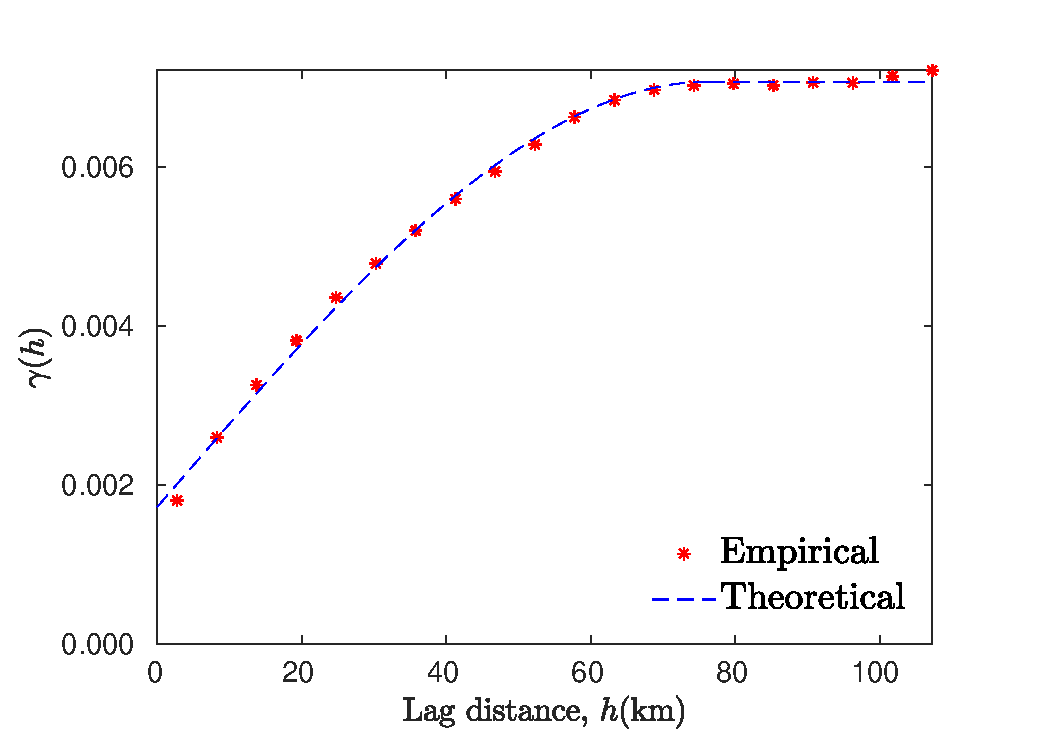
\includegraphics[width=8.5cm]{fig/SemivariogramNDVI225x2251}
\endce
\caption{Averaged in time NDVI semivariogam $\gamma(h)$.}
\label{fig:semivariance}
\end{figure}

\begin{figure}[!htbp]
\begin{center}
\includegraphics[width=0.8\columnwidth]{fig/point50_160GG}
\vspace*{-0.2in}
\caption{SR1-Wavelet decomposition: grid location $(50,160)$. 
Column ($a$) shows the standardized LHI for ANUSPLINE at $6$ decomposition levels using procedure in Section \ref{subsubsec:3_1}. Here $\text{rain}$ represent the values of ANUSPLINE, and $\mu$ and $\sigma$ are the mean and standard deviation of the time series at the grid location. Column ($b$) shows the same $6$ decompositions levels but for standardized NDVI, where $\text{rain} = \text{NDVI}$.}
\label{fig:level_decomposition1}
\end{center}
\end{figure}

\vspace*{-0.2in}
\begin{figure}[!htbp]
\begin{center}
\includegraphics[width=0.8\columnwidth]{fig/point200_20GG}
\vspace*{-0.2in}
\caption{SR1-Wavelet decomposition: grid location $(200,20)$. 
Column ($a$) shows the standardized LHI for ANUSPLINE at $6$ decomposition levels using procedure in Section \ref{subsubsec:3_1}. Here $\text{rain}$ represent the values of ANUSPLINE, and $\mu$ and $\sigma$ are the mean and standard deviation of the time series at the grid location. Column ($b$) shows the same $6$ decompositions levels but for standardized NDVI, where $\text{rain} = \text{NDVI}$.}
\label{fig:level_decomposition2}
\end{center}
\end{figure}

\begin{figure}[!htbp]
\begin{center}
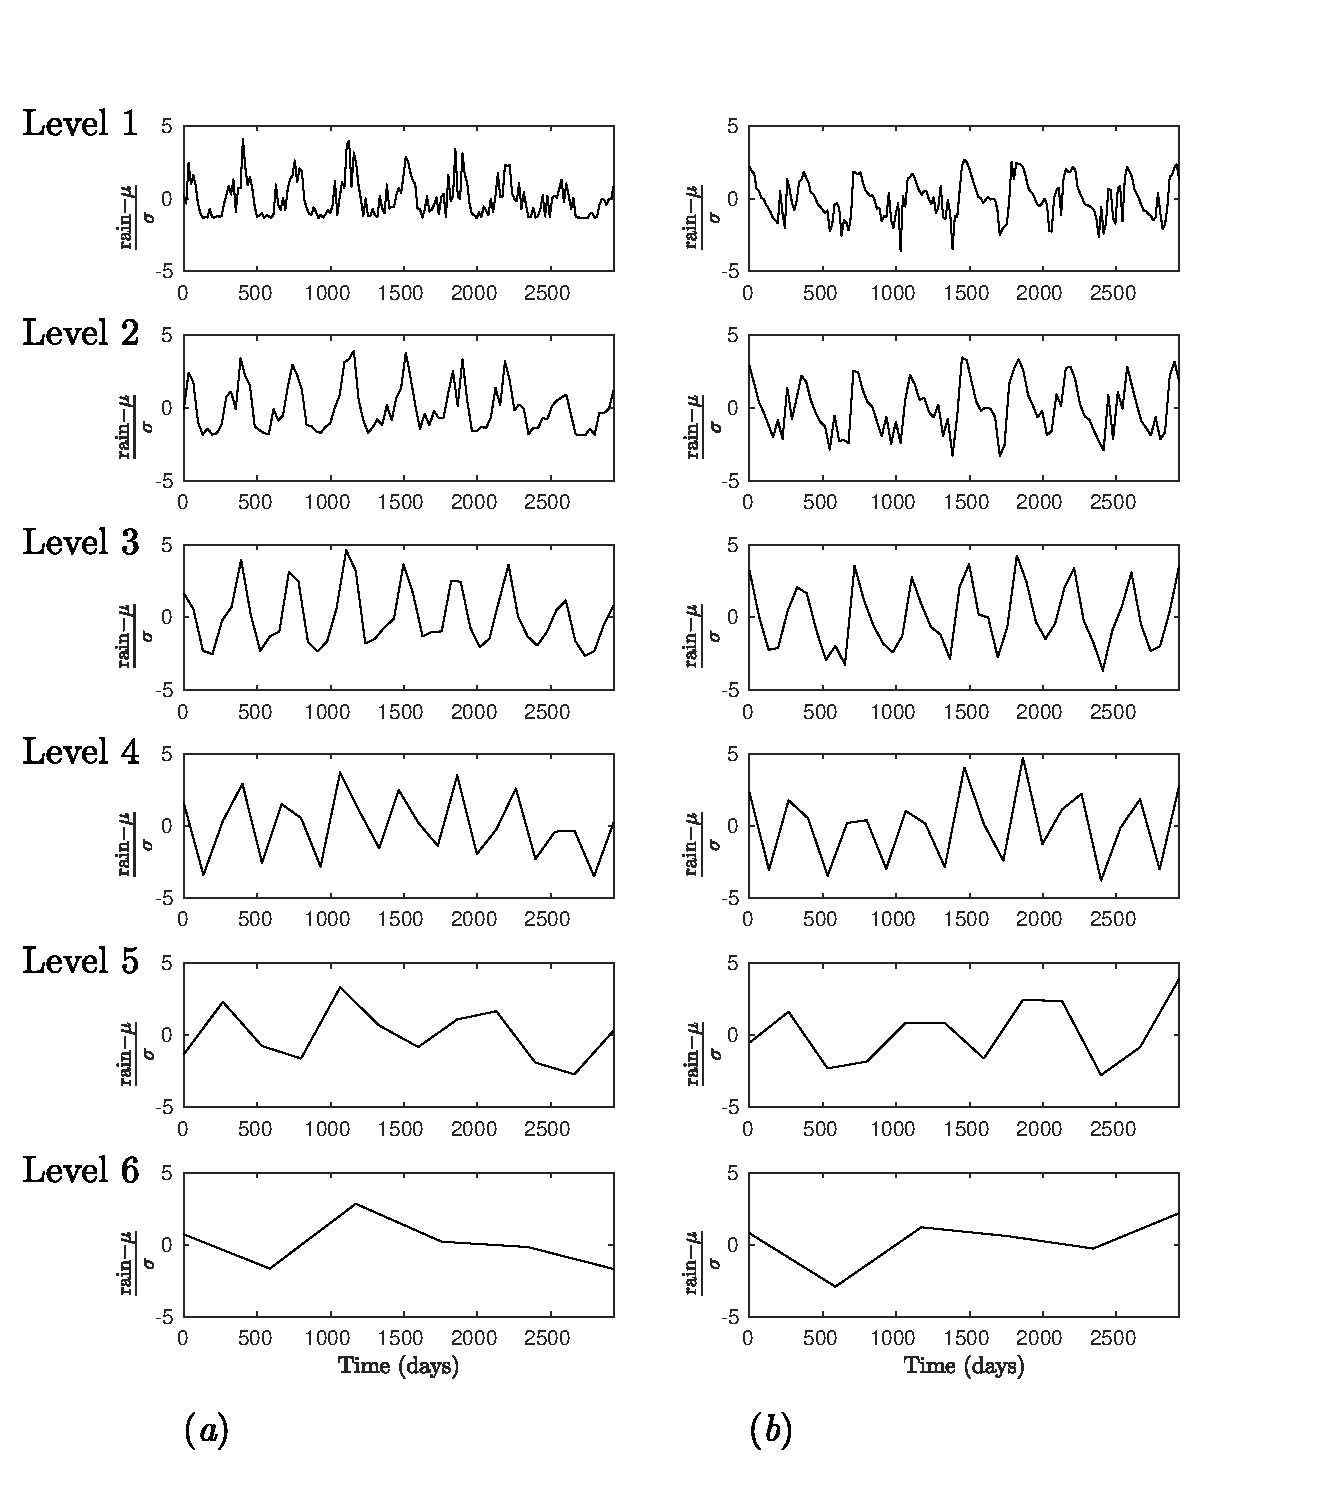
\includegraphics[width=0.8\columnwidth]{fig/point50_160KrigingGG}
\vspace*{-0.2in}
\caption{SR2-Wavelet decomposition: grid location $(50,160)$. 
Column ($a$) shows the standardized LHI for $\bm{\hat{X}}$ at $6$ decomposition levels using procedure in Section \ref{subsubsec:3_1}. Here $\text{rain} = \bm{\hat{X}}$, and $\mu$ and $\sigma$ are the mean and standard deviation of the time series at the grid location. Column ($b$) shows the same $6$ decompositions levels but for standardized NDVI, where $\text{rain} = \text{NDVI}$.}
% Column ($a$) shows standardized $\hat{X}$ and column ($b$) standardized NDVI.}
\label{fig:level_decomposition5}
\end{center}
\end{figure}

\begin{figure}[!htbp]
\begin{center}
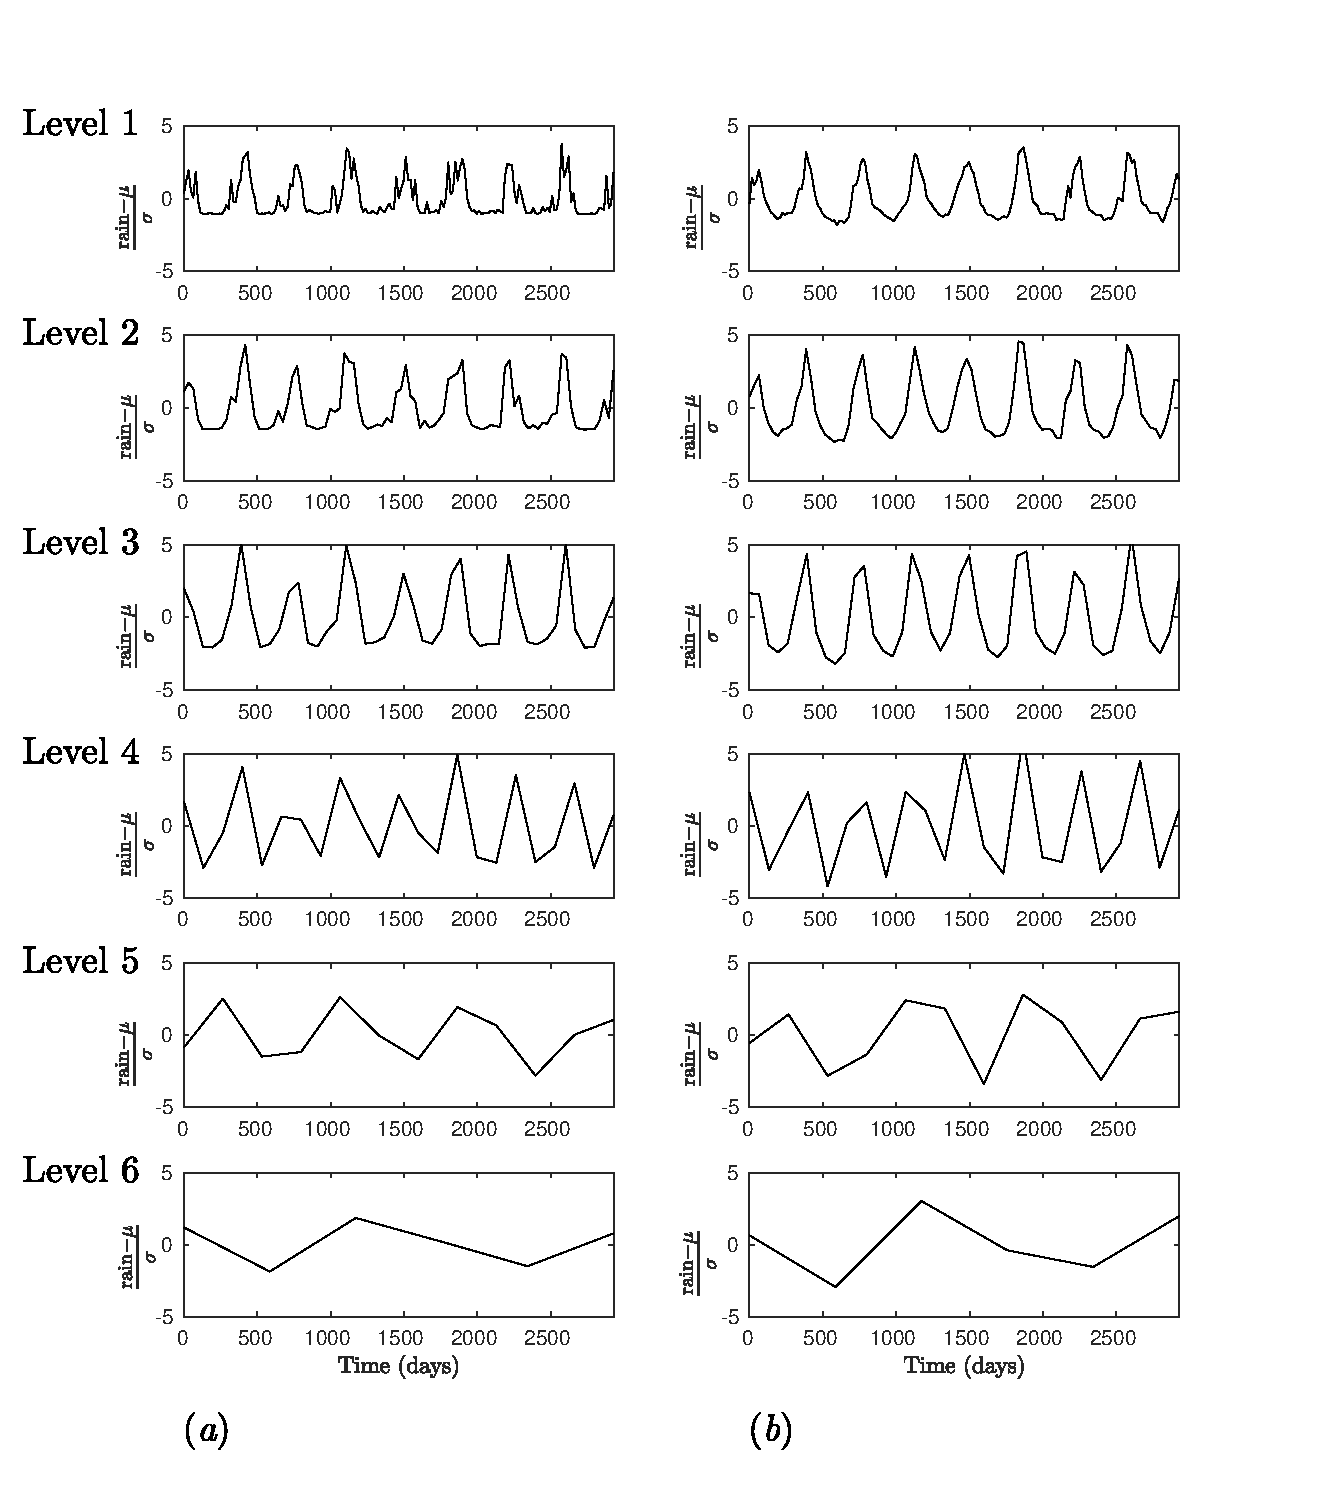
\includegraphics[width=0.8\columnwidth]{fig/point200_20KrigingGG}
\vspace*{-0.2in}
\caption{SR2-Wavelet decomposition: grid location $(200,20)$. 
Column ($a$) shows the standardized LHI for $\bm{\hat{X}}$ at $6$ decomposition levels using procedure in Section \ref{subsubsec:3_1}. Here $\text{rain} = \bm{\hat{X}}$, and $\mu$ and $\sigma$ are the mean and standard deviation of the time series at the grid location. Column ($b$) shows the same $6$ decompositions levels but for standardized NDVI, where $\text{rain} = \text{NDVI}$.}
%Column ($a$) shows standardized $\hat{X}$ and column ($b$) standardized NDVI.}
\label{fig:level_decomposition6}
\end{center}
\end{figure}


\vspace*{-0.5in}
\begin{figure}[!htbp]
	\begce
	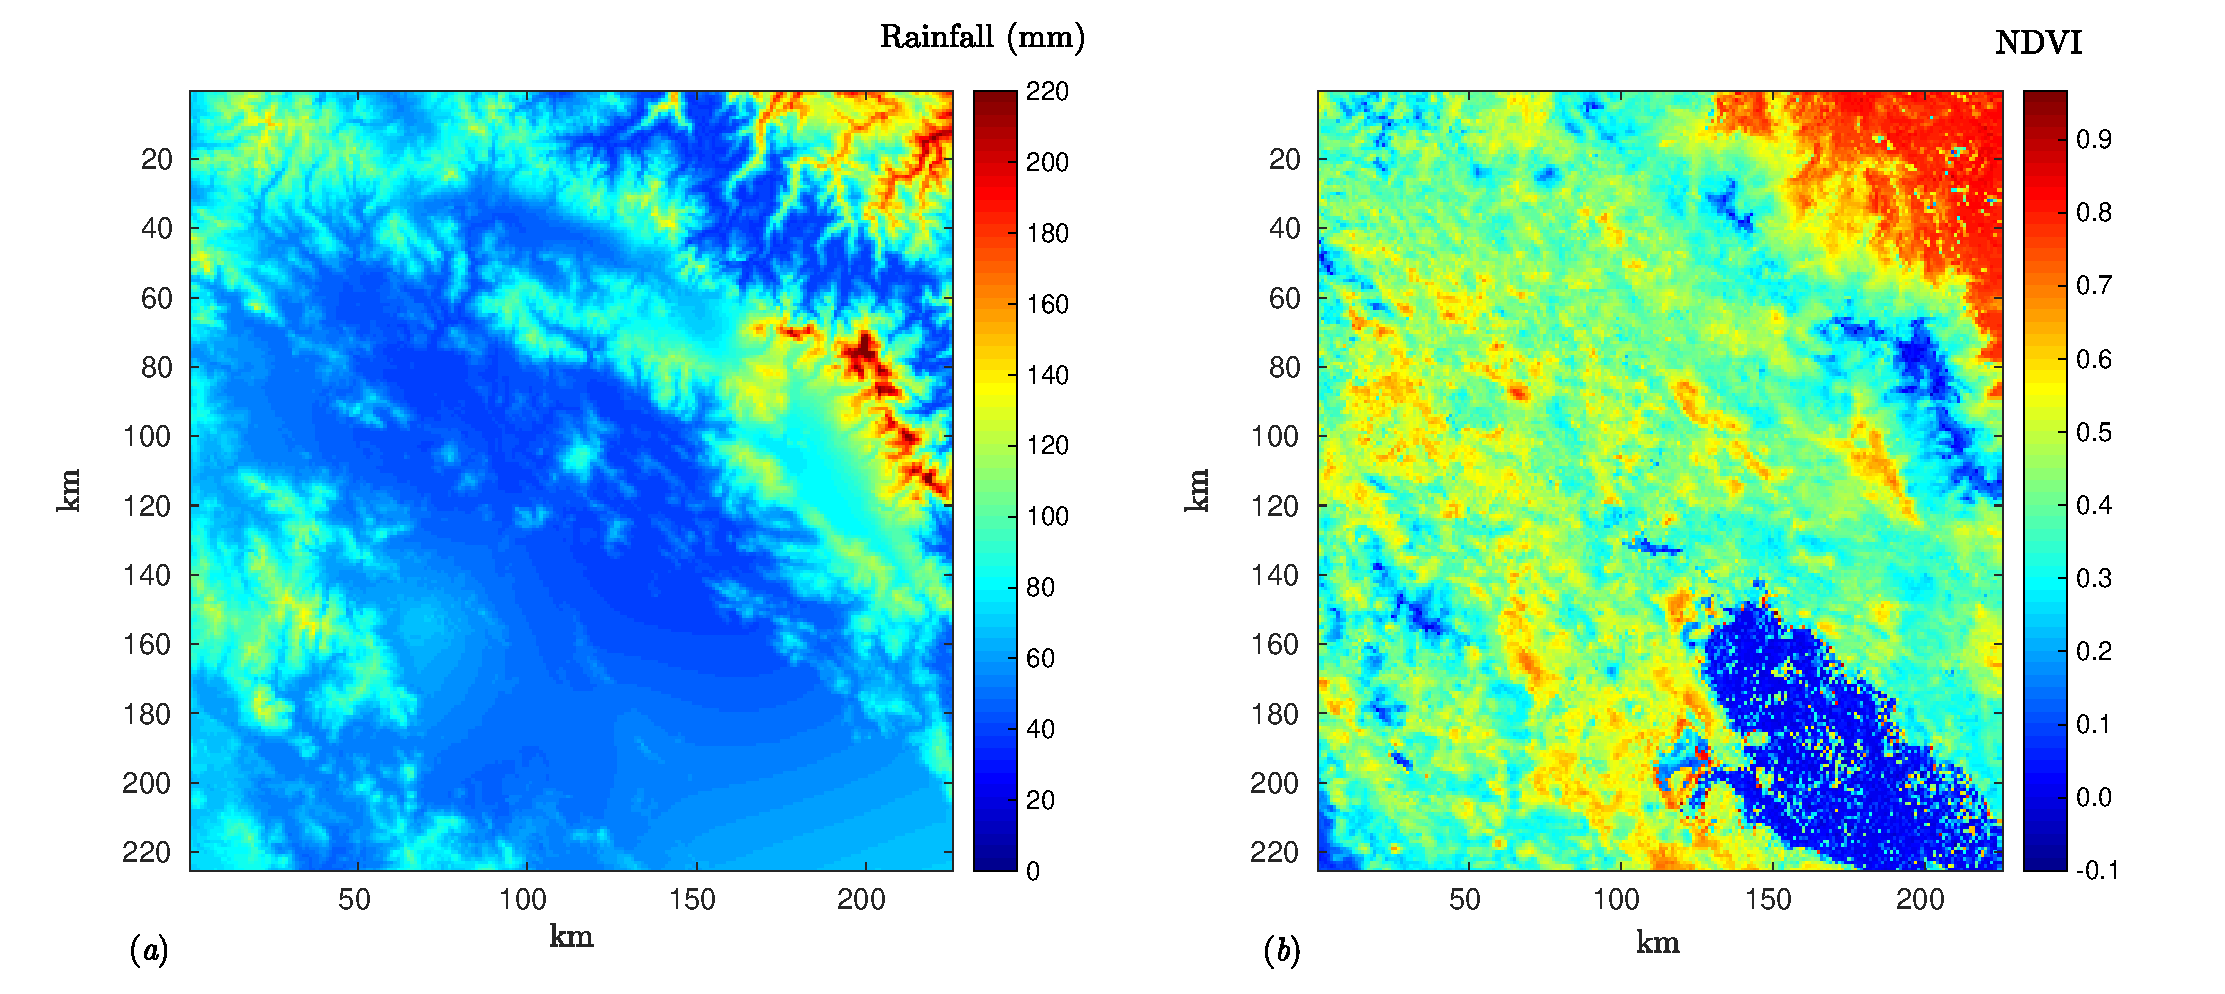
\includegraphics[width=\columnwidth]{fig/NDVI_ANUSPLINE}
	\endce
	\caption{($a$) Rainfall field obtained via ANUSPLINE interpolation for 28 January 2000. ($b$) VGT-S10 NDVI for 28 January 2000. %Colorbar for ($b$) is adimensional since the values are coming from equation  \eqref{eq:NDVI_definition}.
	}
	\label{fig:NDVI_ANUSLINE}
\end{figure}



\begin{figure}[!htbp]
\begce
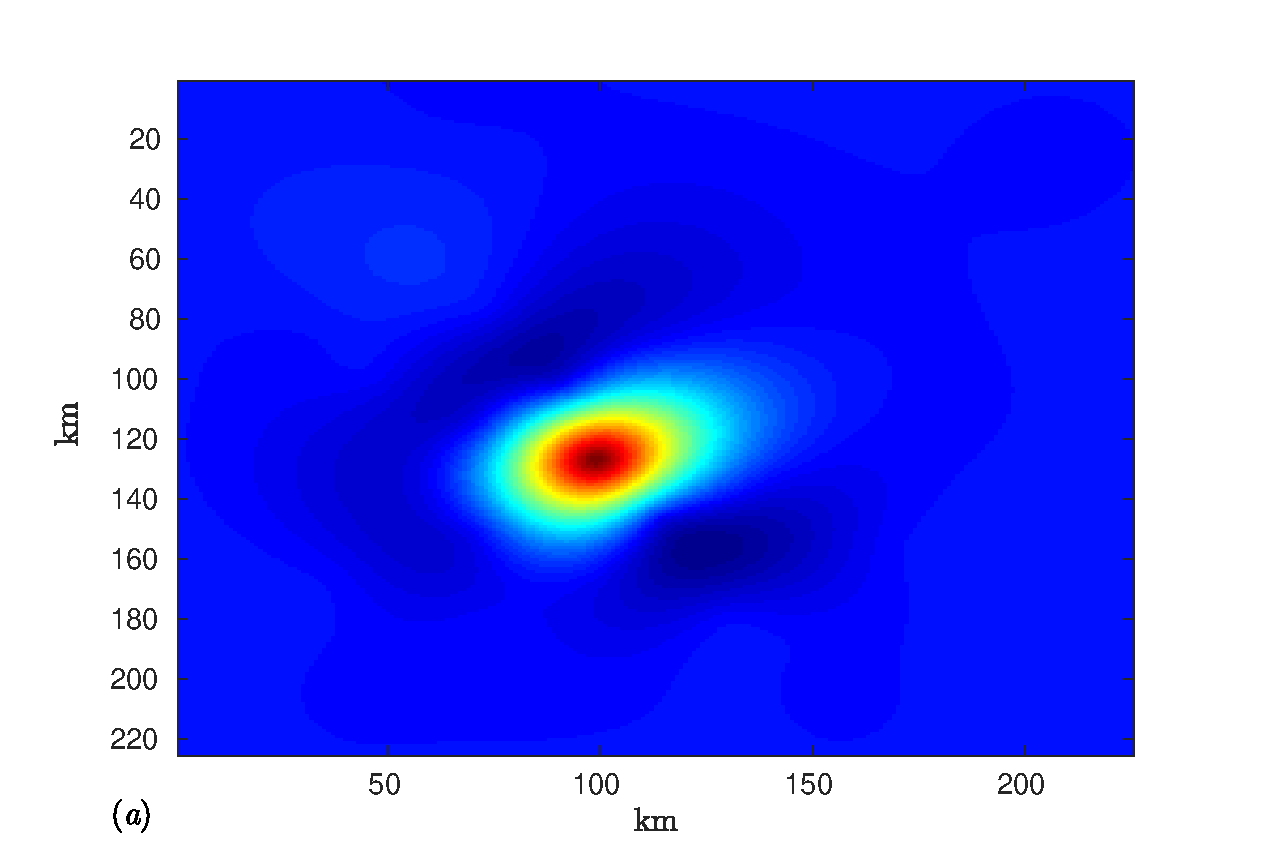
\includegraphics[width=0.5\columnwidth]{fig/AreaweightArapa0}\hspace*{-0.2in}
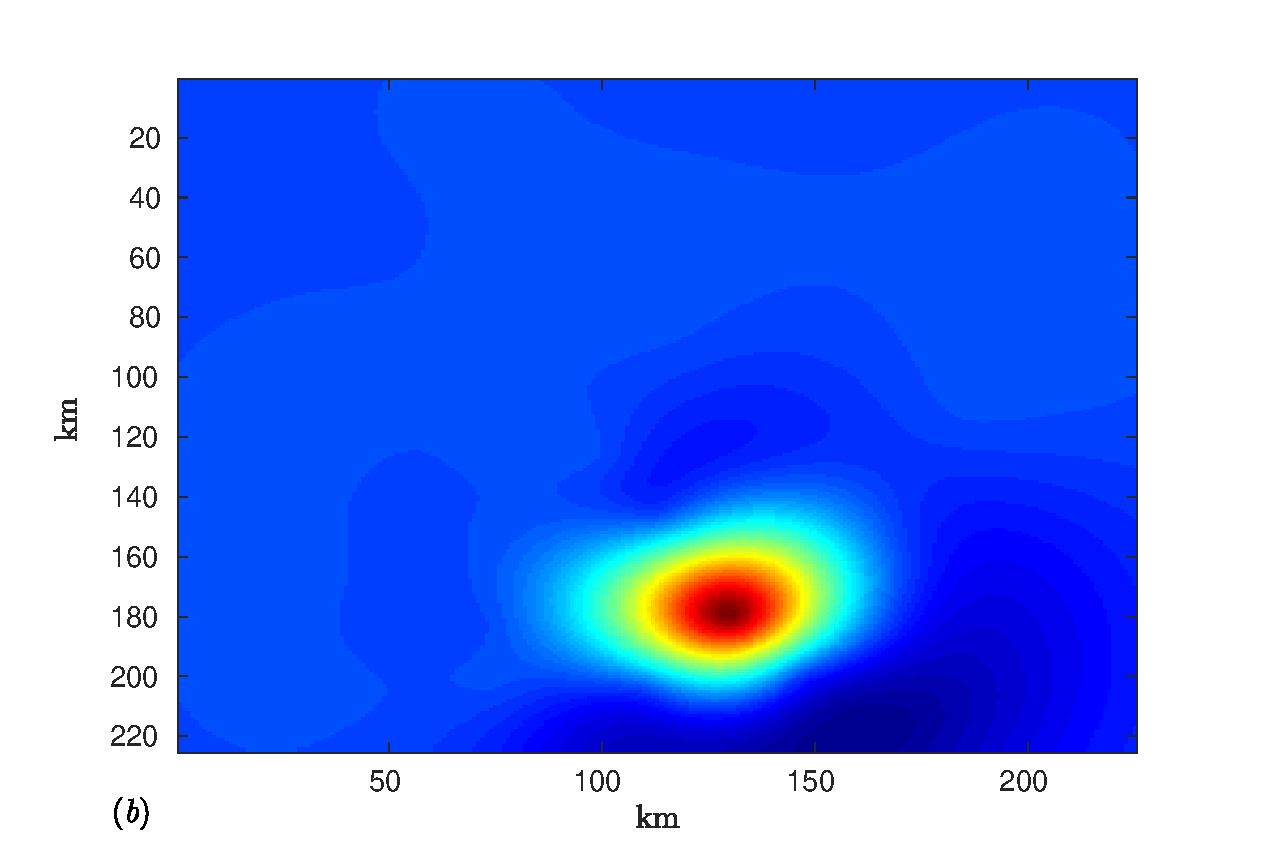
\includegraphics[width=0.5\columnwidth]{fig/AreaweightCapachica0}\\
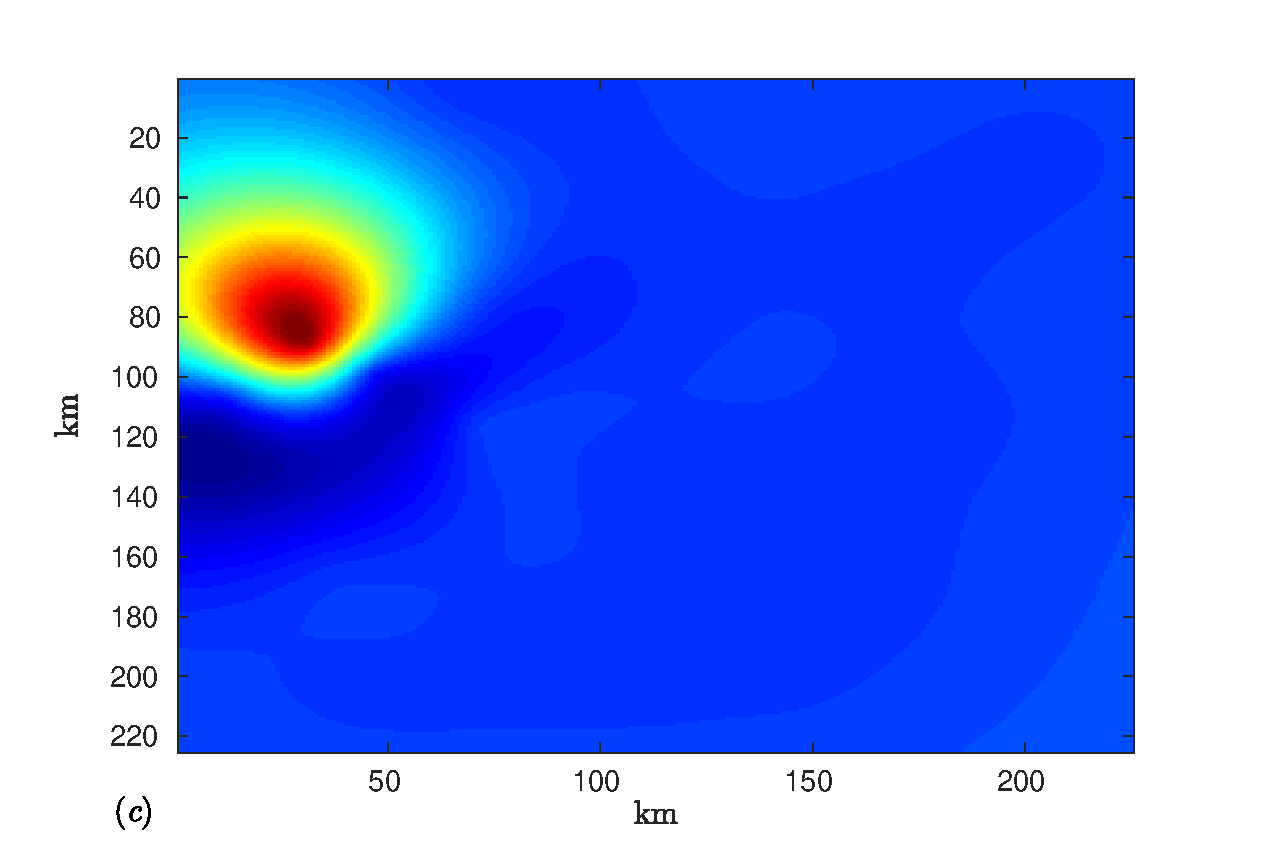
\includegraphics[width=0.5\columnwidth]{fig/AreaweightChuquibambilla0}\hspace*{-0.2in}
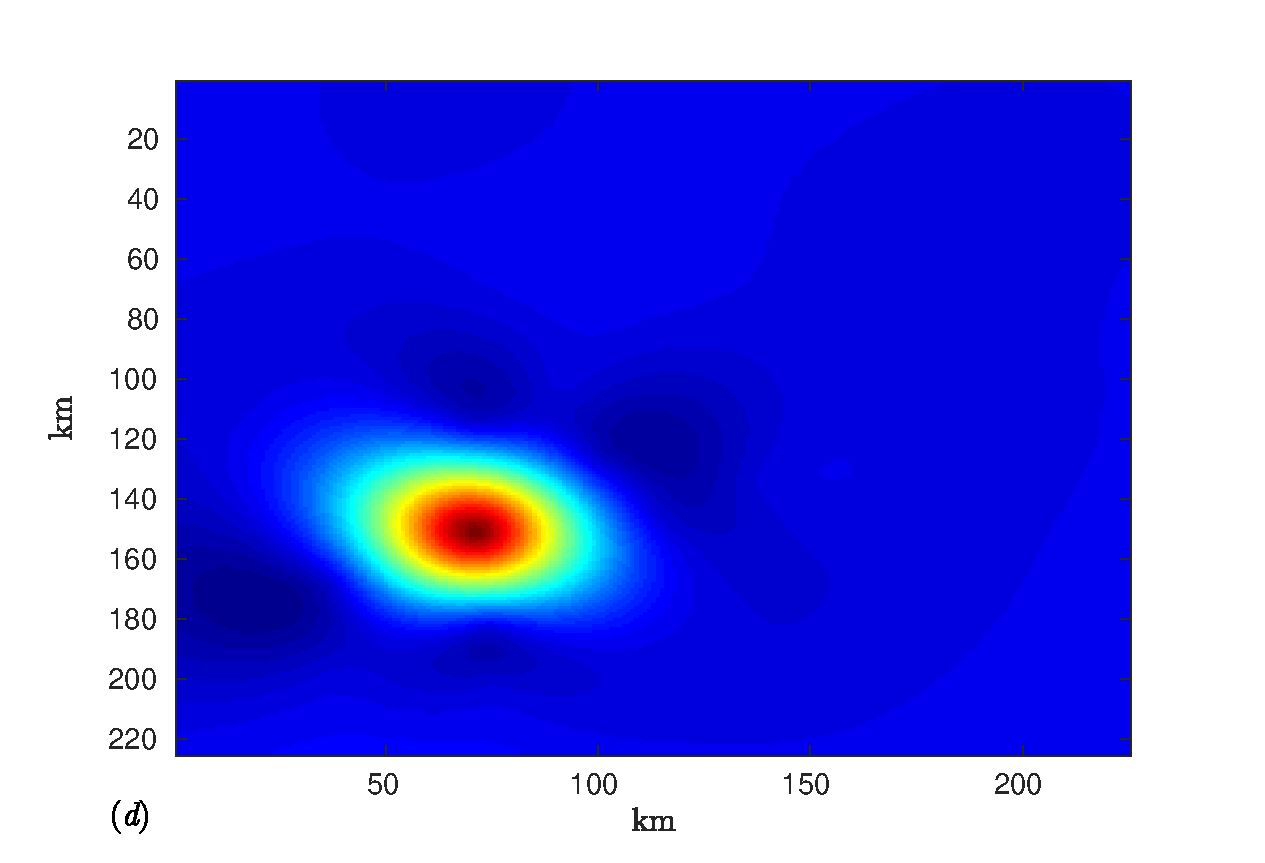
\includegraphics[width=0.5\columnwidth]{fig/AreaweightLampa0} \\
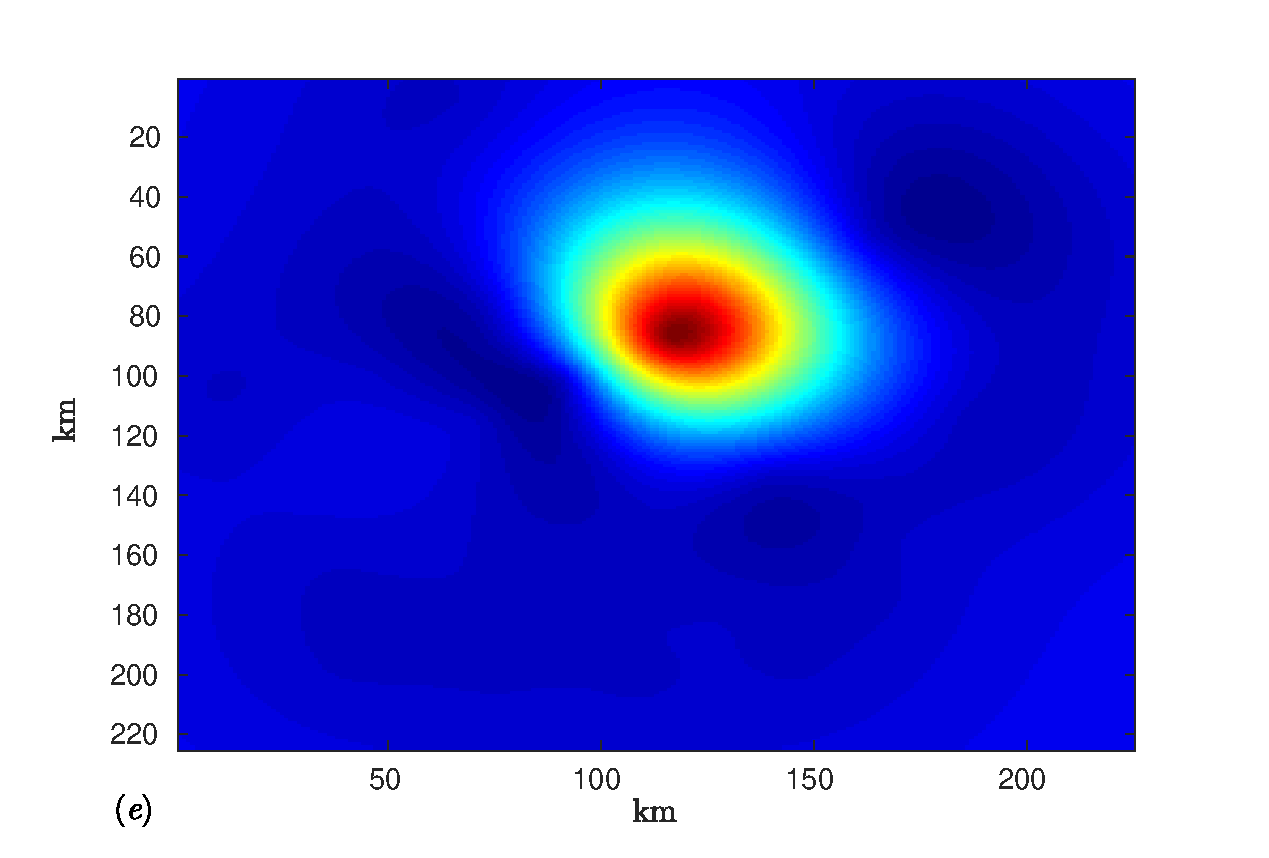
\includegraphics[width=0.5\columnwidth]{fig/AreaweightMunani0}\hspace*{-0.2in}
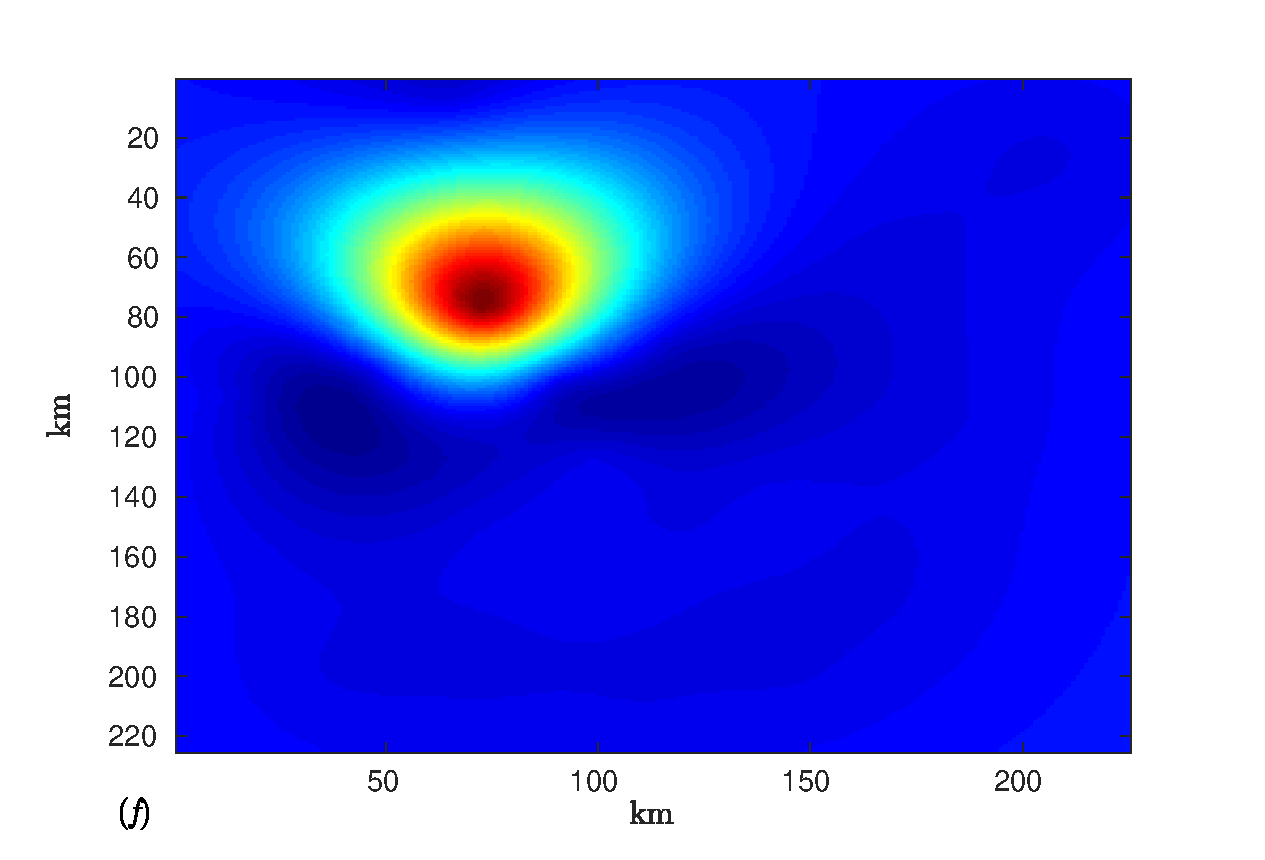
\includegraphics[width=0.5\columnwidth]{fig/AreaweightProgreso0}\\
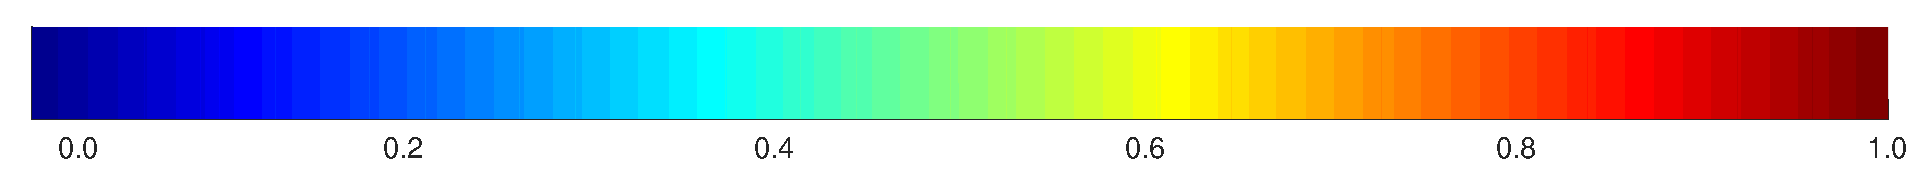
\includegraphics[width=0.8\columnwidth]{fig/colorbar}
\endce
\caption{Spatial lambda values. Each image plots the spatial distribution of 
$\lambda_i$ corresponding to station $i$. First row shows
influence regions for ($a$) Arapa and ($b$) Capachica, second row shows influence regions for ($c$) Chuquibambilla and ($d$) Lampa stations, and third row shows influence regions for ($e$) Munani and ($f$) Progreso stations. The colorbar is adimensional since it represents weights obtained from equation \eqref{eq:lambdaKRIG} at each station and each location in the study area.}
\label{fig:LambdaImages}
\end{figure}

\begin{figure}[!htbp]
\begce
\hspace*{-0.8in}\includegraphics[width=1.3\columnwidth]{fig/ComparisonNDVIscaling1_1_1999EE}\\
\hspace*{-0.8in}\includegraphics[width=1.3\columnwidth]{fig/ComparisonNDVIscaling27_5_2000EE}\\ 
\hspace*{-0.8in}\includegraphics[width=1.3\columnwidth]{fig/ComparisonNDVIscaling9_1_2002EE}\\
\hspace*{-0.8in}\includegraphics[width=1.3\columnwidth]{fig/ComparisonNDVIscaling6_12_2006EE}
$\mbox{({\it{a}})}$   \hspace*{1.7in}   $\mbox{({\it{b}})}$ \hspace*{1.9in} $\mbox{({\it{c}})}$
\endce
\caption{Comparison of methodologies: Column ($a$) SR1, column ($b$) gives the result using Thiessen polygons spatial influence and column ($c$) SR2.}
\label{fig:3methodsComparison}
\end{figure}
\begin{figure}[ht]
\begce
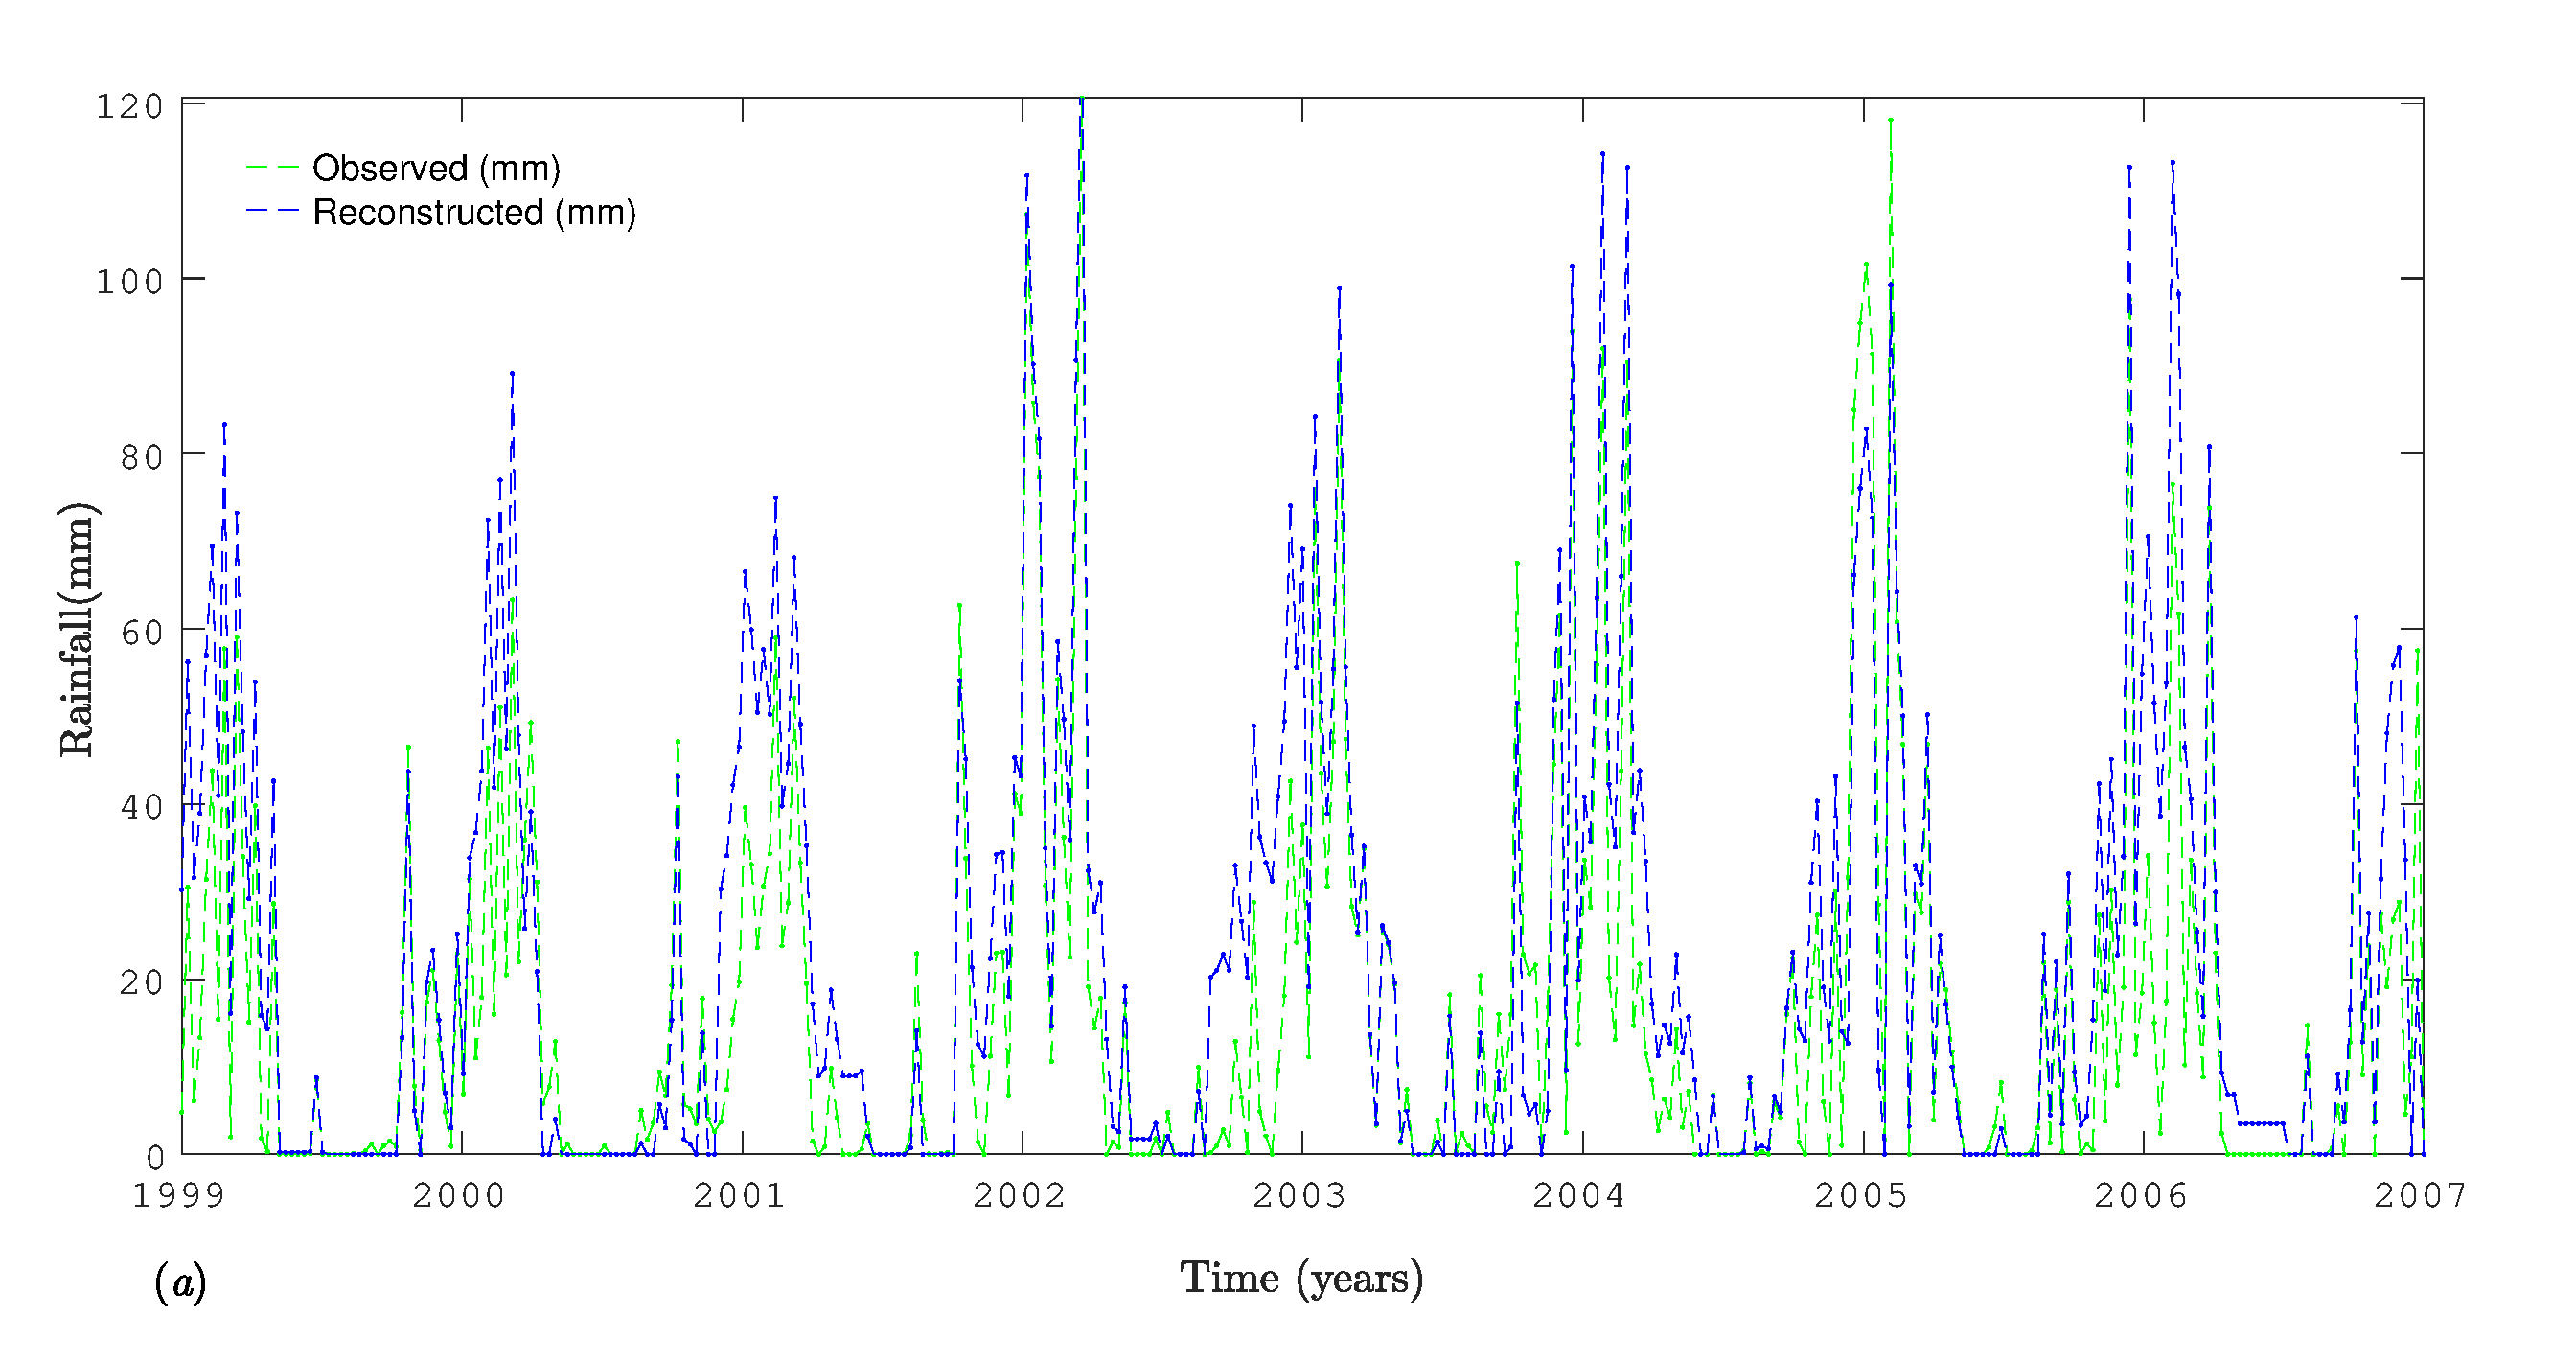
\includegraphics[width=\columnwidth]{fig/TimeSeriesComparisonPucara}\\[0.4in]
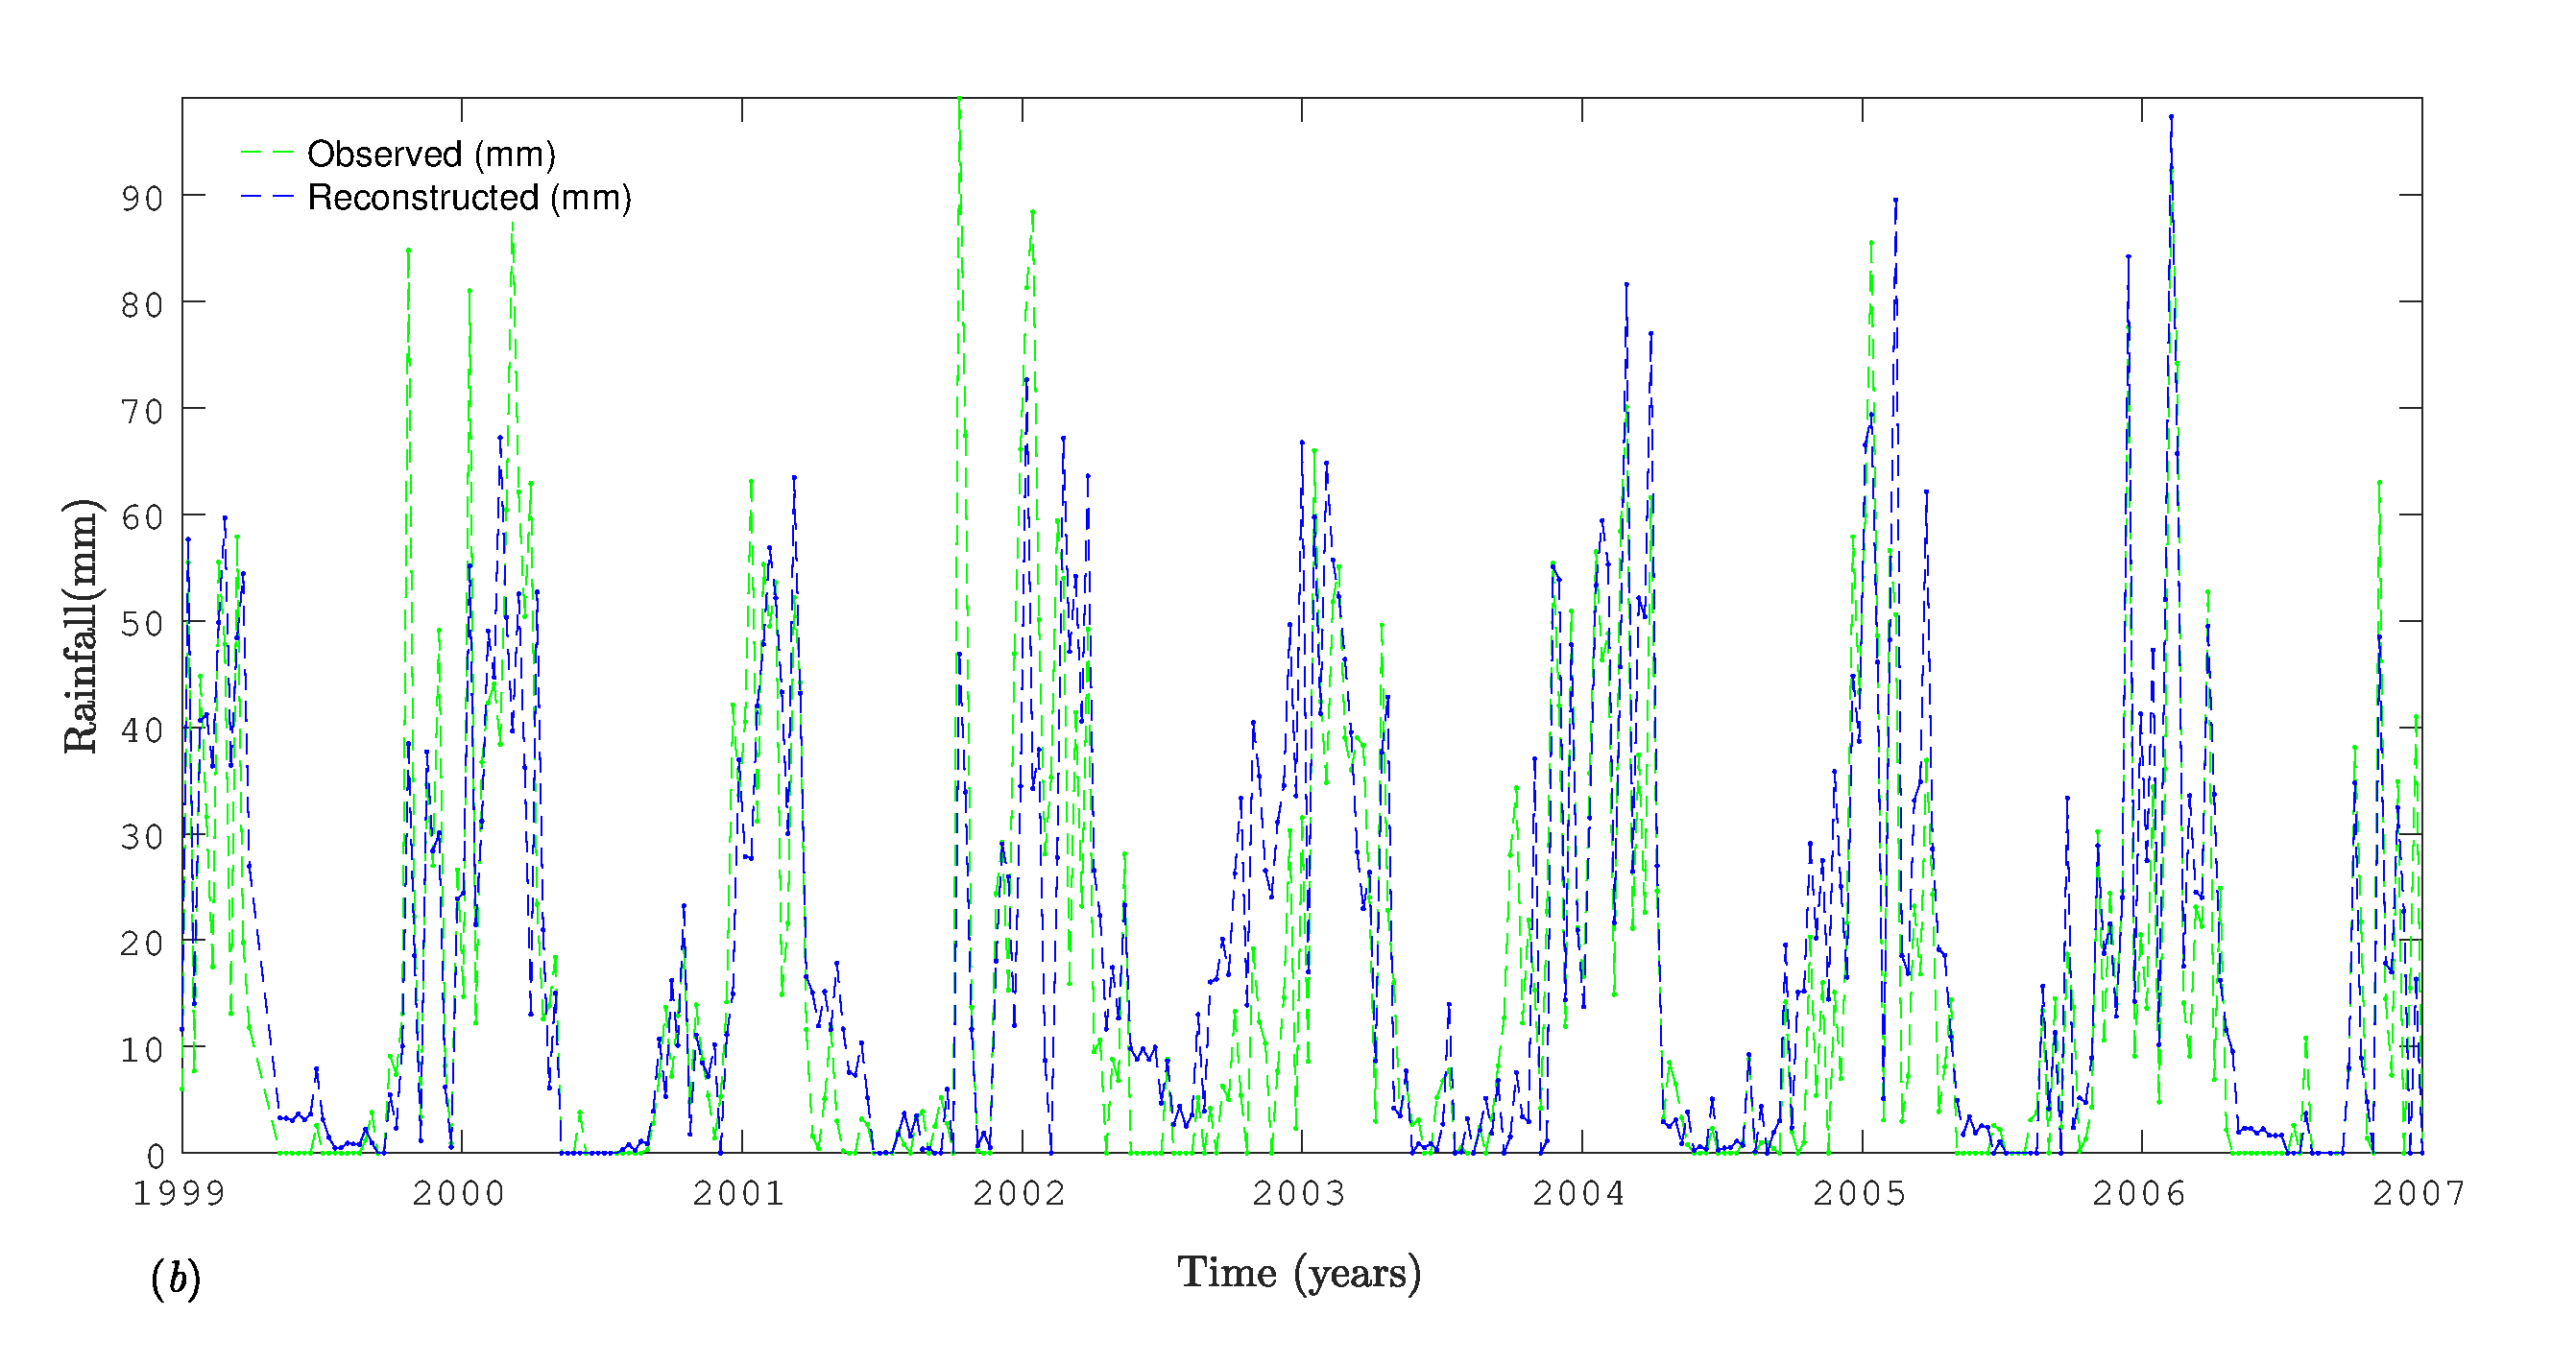
\includegraphics[width=\columnwidth]{fig/TimeSeriesComparisonSantaRosa}
\endce
\caption{Observed and reconstructed precipitation time series: Pucara station ($a$) and Santa Rosa station ($b$). Each rainfall data point  is the result of an $8$ day accumulation period as described in Section \ref{subsubsec:2_2}.}
\label{fig:PucStaRosTimeSeries}
\end{figure}
\begin{figure}[ht]
\begce
\includegraphics[width=\columnwidth]{fig/ECDFcomparisonPucaraN2}\\
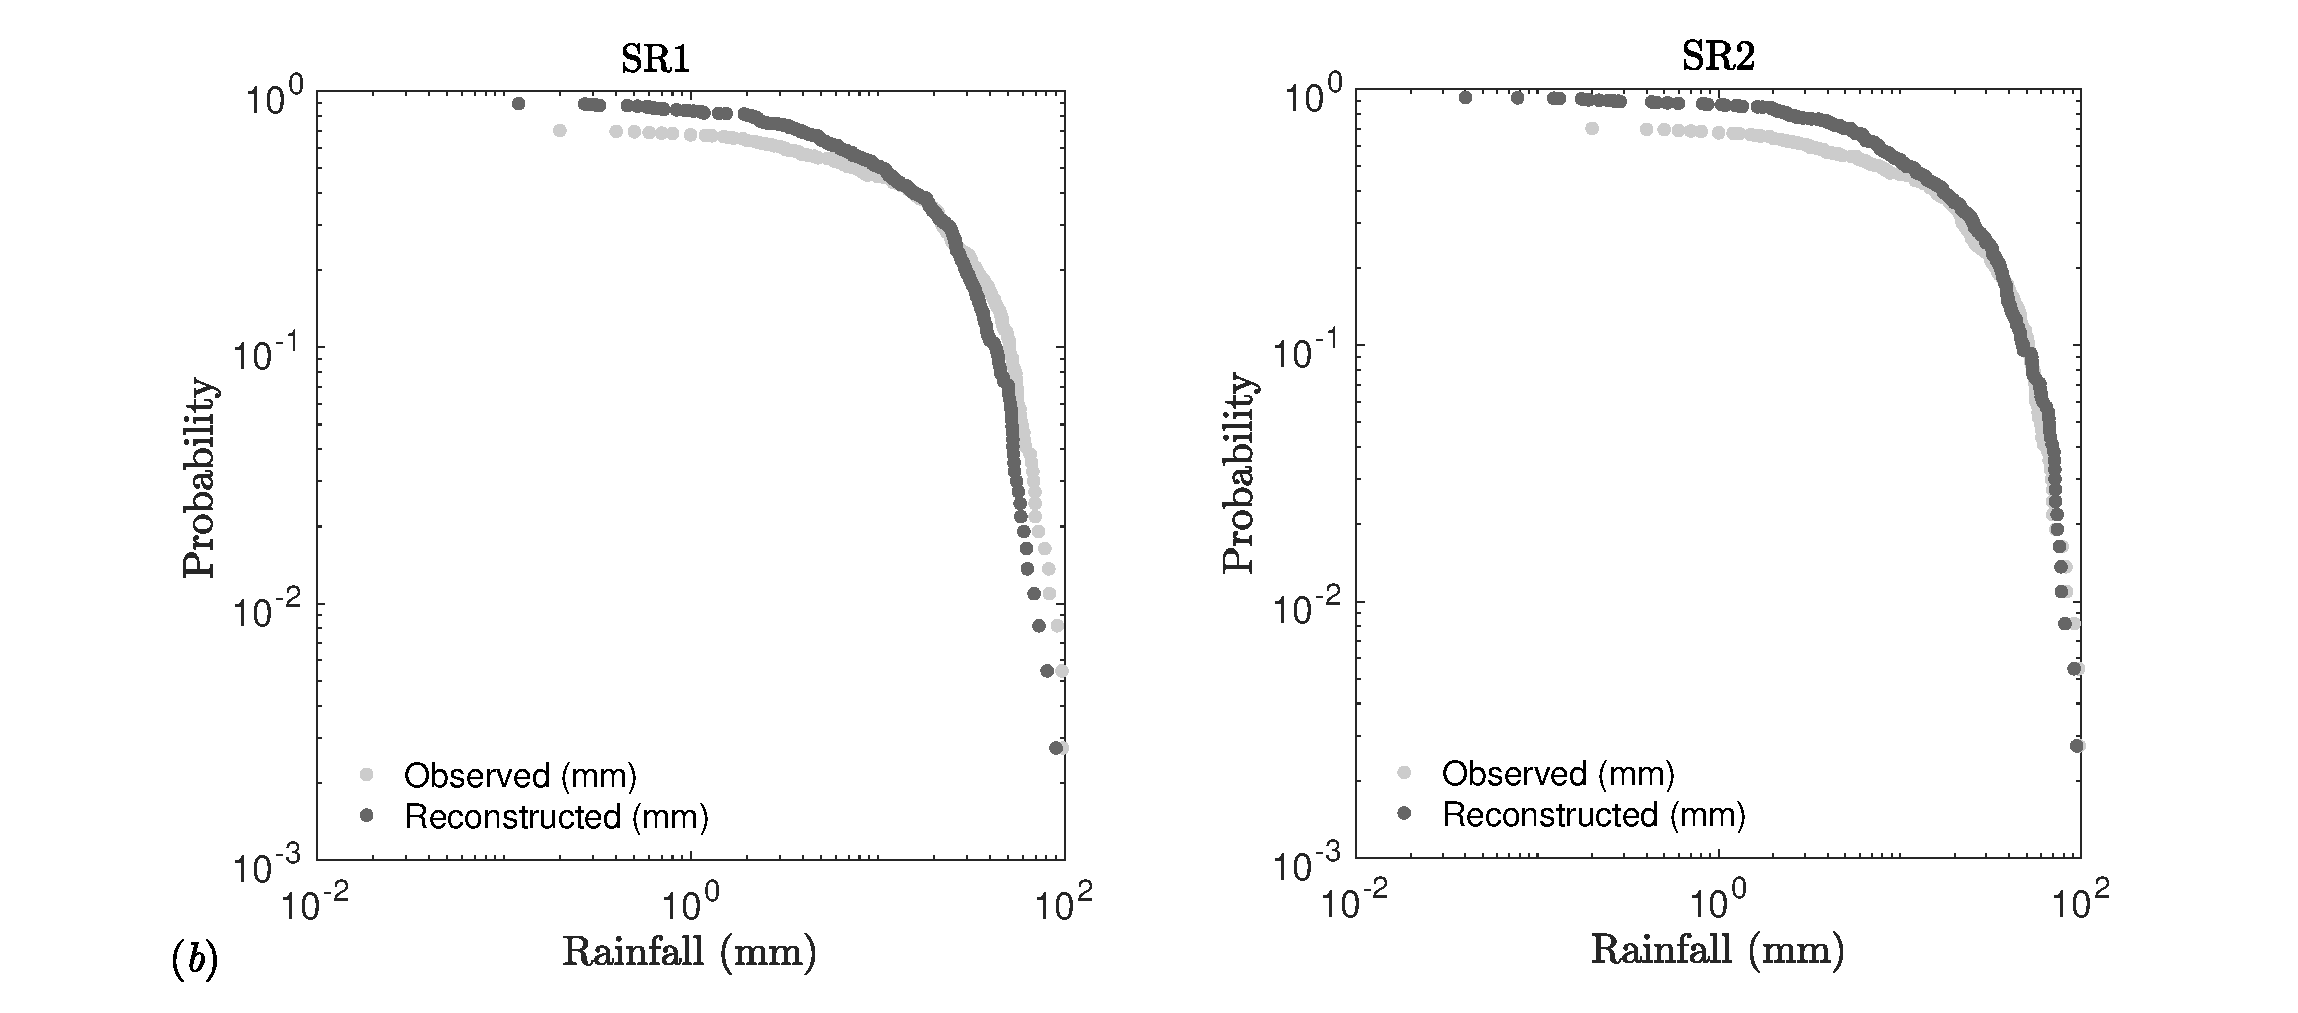
\includegraphics[width=\columnwidth]{fig/ECDFcomparisonSantaRosaN2}
\endce
\caption{Exceedance probability comparison ($8$ day resolution): ($a$) Pucara and ($b$) Santa Rosa.}
\label{fig:3methodsComparison3}
\end{figure}

\end{document}
